\documentclass[12pt,letterpaper,twoside,openright]{report}
%\usepackage{geometry} 
\RequirePackage{amsmath}
\usepackage[spanish]{babel}
\usepackage[latin1]{inputenc} %help babel
%\usepackage{listings}

\usepackage{amssymb}
\usepackage{epstopdf}
\usepackage{longtable}
\usepackage{color}
\usepackage{indentfirst}
\usepackage{algorithm}
\usepackage{algorithmic}
\usepackage[table]{xcolor}
\usepackage{caption}

% to include pdf cover page
\usepackage{pdfpages}

\numberwithin{algorithm}{section}
\newcommand{\theHalgorithm}{\arabic{algorithm}}

\usepackage{hyperref}
\hypersetup{
  pdfborder={0,0,0}
}

%Margins:

%% Commented to accept double sided 

\hoffset=-0.41in %1.5cm left margin: 1in - 0.41in
\marginparwidth = 3cm %3.0cm margin notes as left margin
\oddsidemargin = 1.6cm
\marginparsep = 0.1cm
\textwidth = 16.5cm %to make right margin 2cm and not margin notes
\voffset=-0.22in %2cm upper margin: 1in - 0.22in
\topmargin = 0.5cm %after upper margin before chapter 2cm+topmargin(3cm)
\headheight = 12pt
\footskip = 0.5cm
\headsep = 25pt
\textheight = 21.11cm %

%Equation numeration
\usepackage{amsmath}
%\numberwithin{equation}{subsection}
\numberwithin{equation}{section}

%Operators:
%Single operator:
% \[
%   \operatorname{arg\,max}_a f(a) 
%   = \operatorname*{arg\,max}_b f(b)
% \]
%
% Common operator:
% \DeclareMathOperator*{\argmax}{arg\,max}
%\[
%  \argmax_c f(c)
% \]

%Linespacing 1.5
\usepackage{setspace}
\onehalfspacing  

%Graphic manipulation
\usepackage{graphicx}
\graphicspath{{./images/}} %images path
\usepackage{float}
%\begin{figure}[h t b p ! H]
% \centering
%   \includegraphics[scale=0.5]{graph}
% \caption{A simple graph image}
%\end{figure}

%For figure wrapping
\usepackage{wrapfig}
%\begin{wrapfigure}{r}{0.5\textwidth}
%  \begin{center}
%    \includegraphics[width=0.48\textwidth]{graph}
%  \end{center}
%  \caption{A gull}
%\end{wrapfigure}


%For subfloats
\usepackage{subfig}
 
%\begin{figure}
%  \centering
%  \subfloat[A gull]{\label{fig:gull}\includegraphics[width=0.3\textwidth]{gull}}                
%  \subfloat[A tiger]{\label{fig:tiger}\includegraphics[width=0.3\textwidth]{tiger}}
%  \subfloat[A mouse]{\label{fig:mouse}\includegraphics[width=0.3\textwidth]{mouse}}
%  \caption{Pictures of animals}
%  \label{fig:animals}
%\end{figure}

%enumeration depth
\setcounter{secnumdepth}{3}

%compile just these 'include' tags
%\includeonly{chapter1,chapter2,chapter3,chapter4,chapter5} 
\includeonly{abstract-spa,chapter1-spa}

\title{Image processing to detect worms}
\author{Javier Fern\'andez}

\begin{document}

\maketitle

%
\includepdf[pages=1]{cover/cover}
%\thispagestyle{empty}
%\cleardoublepage
%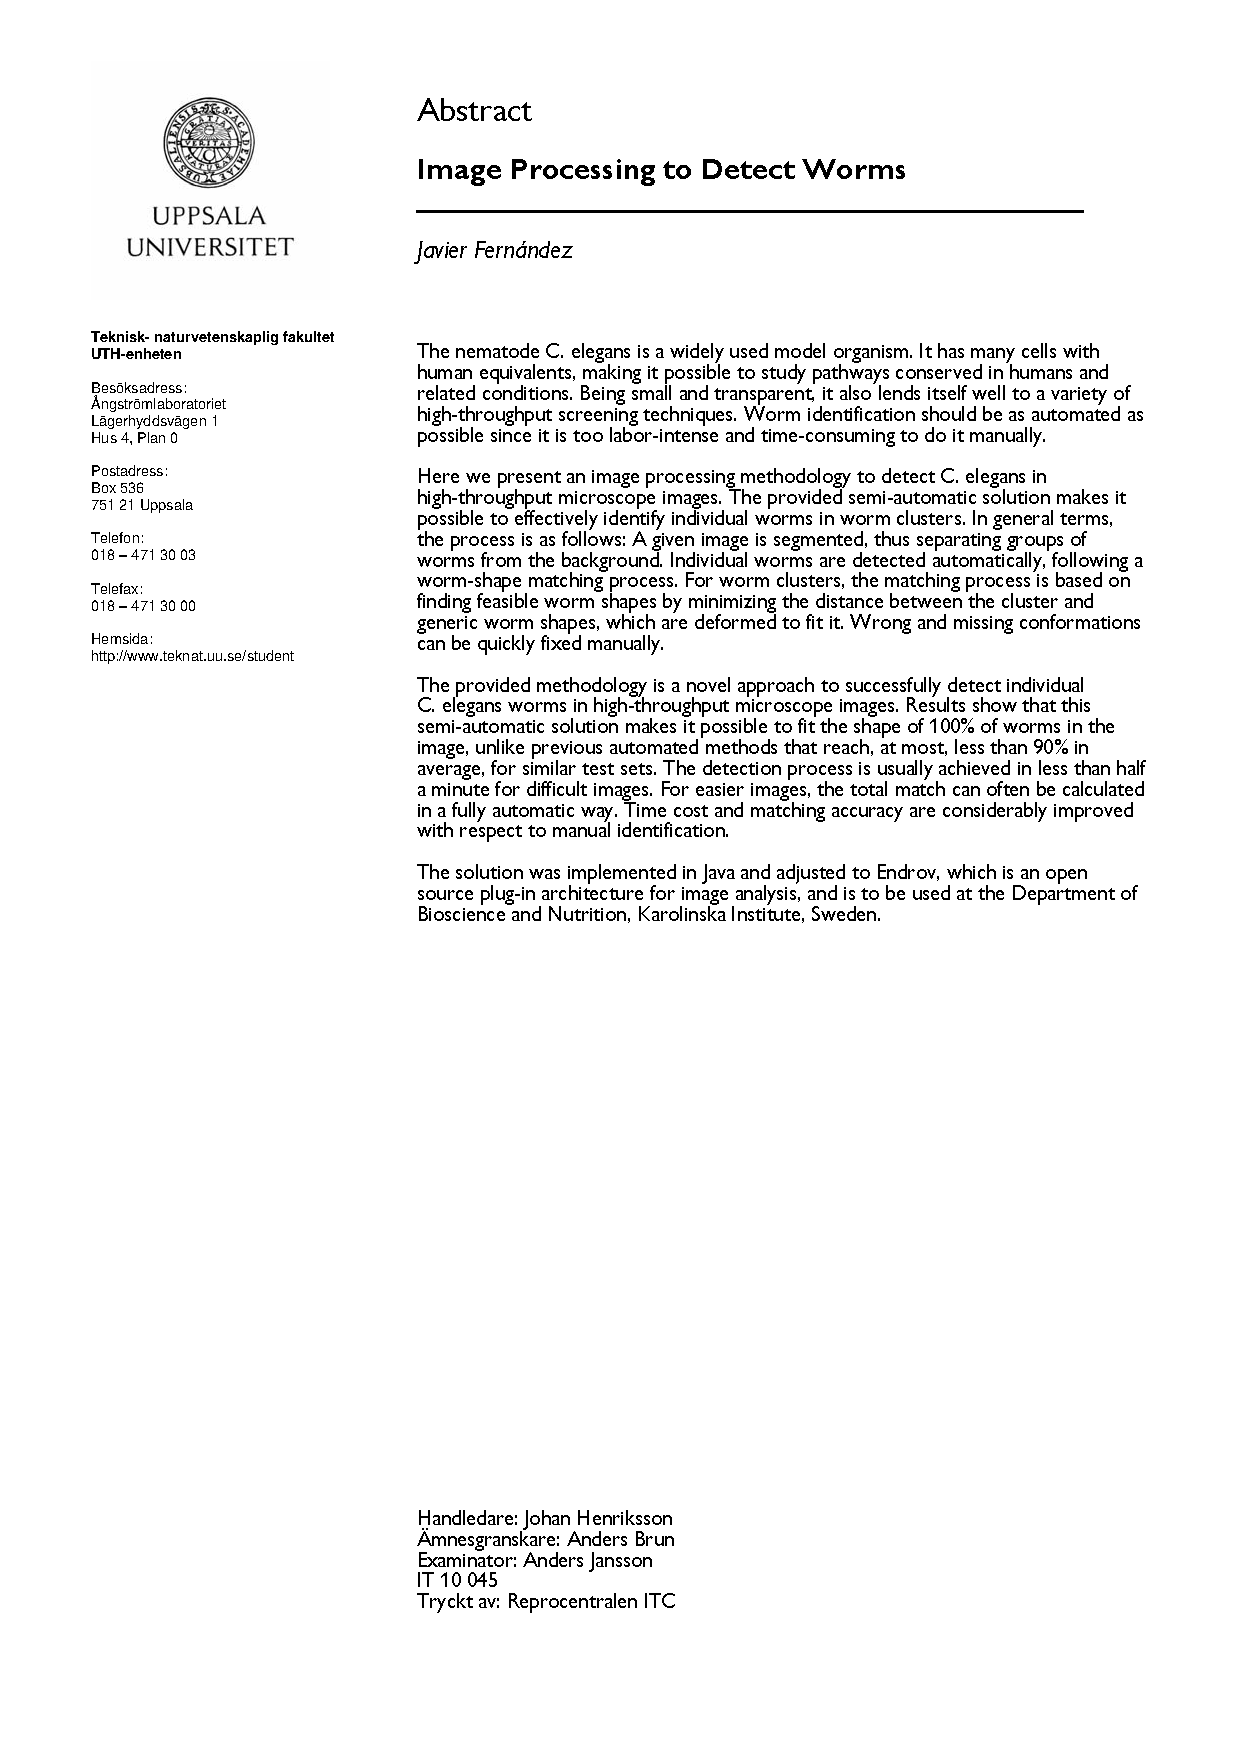
\includepdf[pages=1]{cover/abstract}
%\thispagestyle{empty}
%\cleardoublepage

%\begin{abstract}

   % What is C. elegans and why is it so important.
   % The problem: manual assays are to intensive, need
   % for automated solutions.
   % What do we provide: a image processing methodology that
   % provides semi-automatic solution, for Endrov (open source
   % image analysis software)
   % Few methods attempt to resolve cluttering. Individual
   % images are not usually addressed (large datasets).
   % Automated solutions fit 85 percent of the image. We 
   % fit 100% 

El nematodo C. elegans es un organismo ampliamente
utilizado. Posee muchas c\'elulas con equivalentes humanos y otras
condiciones especialmente favorables, que lo han convertido en modelo
de estudio para la biolog\'ia, especialmente la g\'enetica del
desarrollo. As\'i mismo, al ser peque\~no y transparente se presta bien
a una gran variedad de t\'ecnicas de cribado de alto rendimiento
(HTS). \\ 

La identificaci\'on de gusanos deber\'ia automatizarse lo mas
posible dado que es muy trabajoso efectuarla manualmente.
En este trabajo se presenta una metodolog\'ia de procesamiento de im\'agenes
para detectar C. elegans en im\'agenes obtenidas por microscop\'ia de 
alto rendimiento. La soluci\'on semi-autom\'atica que aqu\'i se provee, permite identificar
eficazmente gusanos particulares en agrupaciones de gusanos. En
t\'erminos generales, el proceso  consta de lo siguiente:
una imagen dada es segmentada, separando as\'i grupos de gusanos del
fondo de la imagen. Se detectan gusanos particulares de manera autom\'atica, siguiendo un
proceso de comparaci\'on y ajuste de siluetas de gusanos. Este proceso
se basa en encontrar siluetas factibles dentro de una agrupaci\'on, 
minimizando la distancia que existe entre dicha agrupaci\'on y 
siluetas gen\'ericas que son deformadas para ajustarse a ella.
Las conformaciones de gusanos ajustadas incorrectamente 
pueden ser corregidas f\'acilmente de manera manual.\\

La metodolog\'ia provista presenta un enfoque innovador para
detectar exitosamente gusanos C. elegans particulares en 
im\'agenes de microscopio. Los resultados muestran que esta soluci\'on
semi-autom\'atica permite detectar, correctamente, la silueta del 100\% de 
los gusanos presentes en una imagen determinada, a diferencia de otros m\'etodos
automatizados que alcanzan a detectar, en promedio, menos del 90\% ,
para conjuntos de pruebas similares.
Por lo general, el proceso es completado en menos de minuto y medio
para im\'agenes dif\'iciles. Para im\'agenes mas sencillas, los gusanos
puede ser identificados en su totalidad de manera enteramente 
autom\'atica. La precisi\'on de la detecci\'on y el tiempo requerido 
para calcularla son mejorados notablemente con respecto a la
idenficaci\'on manual.\\

La soluci\'on fue implementada en \emph{Java} e integrada a
\emph{Endrov}, una arquitectura de extensiones de c\'odigo abierto para
an\'alisis de im\'agenes, y ser\'a utilizada en el Departamento de
  Biociencias y Nutrici\'on del Instituto Karolinksa, Suecia.

\end{abstract}


\pagenumbering{roman}
\setcounter{page}{1}
\tableofcontents
\listoffigures
\listoftables
%must be below \tableofcontents: paragraph indentation
\setlength{\parindent}{10pt} %look for 3-spaces in late
\begin{abstract}

   % What is C. elegans and why is it so important.
   % The problem: manual assays are to intensive, need
   % for automated solutions.
   % What do we provide: a image processing methodology that
   % provides semi-automatic solution, for Endrov (open source
   % image analysis software)
   % Few methods attempt to resolve cluttering. Individual
   % images are not usually addressed (large datasets).
   % Automated solutions fit 85 percent of the image. We 
   % fit 100% 

El nematodo C. elegans es un organismo ampliamente
utilizado. Posee muchas c\'elulas con equivalentes humanos y otras
condiciones especialmente favorables, que lo han convertido en modelo
de estudio para la biolog\'ia, especialmente la g\'enetica del
desarrollo. As\'i mismo, al ser peque\~no y transparente se presta bien
a una gran variedad de t\'ecnicas de cribado de alto rendimiento
(HTS). \\ 

La identificaci\'on de gusanos deber\'ia automatizarse lo mas
posible dado que es muy trabajoso efectuarla manualmente.
En este trabajo se presenta una metodolog\'ia de procesamiento de im\'agenes
para detectar C. elegans en im\'agenes obtenidas por microscop\'ia de 
alto rendimiento. La soluci\'on semi-autom\'atica que aqu\'i se provee, permite identificar
eficazmente gusanos particulares en agrupaciones de gusanos. En
t\'erminos generales, el proceso  consta de lo siguiente:
una imagen dada es segmentada, separando as\'i grupos de gusanos del
fondo de la imagen. Se detectan gusanos particulares de manera autom\'atica, siguiendo un
proceso de comparaci\'on y ajuste de siluetas de gusanos. Este proceso
se basa en encontrar siluetas factibles dentro de una agrupaci\'on, 
minimizando la distancia que existe entre dicha agrupaci\'on y 
siluetas gen\'ericas que son deformadas para ajustarse a ella.
Las conformaciones de gusanos ajustadas incorrectamente 
pueden ser corregidas f\'acilmente de manera manual.\\

La metodolog\'ia provista presenta un enfoque innovador para
detectar exitosamente gusanos C. elegans particulares en 
im\'agenes de microscopio. Los resultados muestran que esta soluci\'on
semi-autom\'atica permite detectar, correctamente, la silueta del 100\% de 
los gusanos presentes en una imagen determinada, a diferencia de otros m\'etodos
automatizados que alcanzan a detectar, en promedio, menos del 90\% ,
para conjuntos de pruebas similares.
Por lo general, el proceso es completado en menos de minuto y medio
para im\'agenes dif\'iciles. Para im\'agenes mas sencillas, los gusanos
puede ser identificados en su totalidad de manera enteramente 
autom\'atica. La precisi\'on de la detecci\'on y el tiempo requerido 
para calcularla son mejorados notablemente con respecto a la
idenficaci\'on manual.\\

La soluci\'on fue implementada en \emph{Java} e integrada a
\emph{Endrov}, una arquitectura de extensiones de c\'odigo abierto para
an\'alisis de im\'agenes, y ser\'a utilizada en el Departamento de
  Biociencias y Nutrici\'on del Instituto Karolinksa, Suecia.

\end{abstract}

%\cleardoublepage
\thispagestyle{empty}
\chapter{INTRODUCCI\'ON}
\pagenumbering{arabic}

\section{Motivaci\'on y Prop\'osito}
\label{sec:motivation}

El nematodo C. elegans es un organismo ampliamente utilizado
y se ha convertido en un importante modelo de estudio para la
biolog�a, especialmente la gen�tica del desarrollo.
Presenta la ventaja de que todos los individuos son exactamente
iguales a nivel celular, poseen cortos ciclos de vidas y una r�pida
gen�tica. Por esta raz�n, se pueden detectar tipos salvajes de este organismo 
y los experimentos son menos costosos, en comparaci�n 
con organismos m�s complejos. Es el �nico animal del que se conoce
cada divisi�n celular, desde la fertilizaci�n del huevo hasta la etapa
adulta, as� como el diagrama completo de las conexiones de esas
c�lulas.\\

El C. elegans tiene muchas c�lulas con equivalentes humanos, lo que 
hace posible estudiar y comprender como se manifiestan ciertas
enfermedades y condiciones relacionadas, e.g. addicci�n a las drogas,
envejecimiento, disfunci�n de ciertas prote�nas, etc.
As� mismo, al ser peque�o y transparente, se presta bien
a una gran variedad de t�cnicas de cribado de alto rendimiento
(HTS). El HTS es un m�todo de experimentaci�n cient�fica que permite
conducir millones de pruebas gen�ticas, bioqu�micas o farmacol�gicas,
a trav\'es de la rob\'otica, softwares de control y procesamiento de datos,
dispositivos para el manejo de l\'iquidos y detectores sensitivos.
A trav�s de este proceso se pueden identificar r�pidamente componentes
activos, anticuerpos o genes que modelan procesos biomoleculares
particulares, tal como se indica en \cite{highthroughput}. \\
Diversos ganadores del premio Nobel de Medicina o Fisiolog�a
han centrado sus estudios en gusanos, y en particular C. elegans, 
tales como Brenner, Sulston y Horvitz (2002), Fire y Mello (2008),
as� como el ganador del Nobel de Qu�mica, Martin Chalfie (2008).\\

Antes de ser cuantificados, los gusanos deben ser identificados. Este
proceso deber�a ser autom�tico debido a que es muy trabajoso para
ser efectuado manualmente en un tiempo factible. Curiosamente, a 
pesar de la utilidad del C. elegans para manipulaciones gen�ticas,
su utilizaci�n en procesos de cribado de alto rendimiento se
ha visto tambi\'en limitado por la necesidad de ensayos manuales 
muy trabajosos.\\

Esto conlleva a la necesidad de m\'etodos mas r\'apidos y consistentes.
Por esta raz\'on, un programa de computadora que permita detectar individuos 
C. elegans en im\'agenes digitales, proveer\'ia una soluci\'on autom\'atica
para el problema de reconocimiento. Esto mejorar\'ia tanto la precisi\'on como 
el tiempo requerido para la identificaci\'on de los individuos, con respecto
a la identificaci\'on manual, permitiendo, a su vez, transformar 
las im\'agenes en informaci\'on manejable.\\

El presente estudio, se centra en el dise\~no e implementaci\'on de un 
algoritmo de procesamiento de im\'agenes para detectar 
gusanos C. elegans en im\'agenes de microscopio. Se provee,
as\'i mismo, una metodolog\'ia general de detecci\'on de gusanos.
La caracter\'istica mas relevante para la 
mayor\'ia de los experimentos con C. elegans es la forma del 
gusano, y en ocasiones tambi\'en la rotaci\'on y direcci\'on de la misma.
El enfoque que aqu\'i se presenta, busca identificar, exclusivamente, 
la forma de los gusanos. Se estudia, entonces, si es posible detectar 
y ajustar estas formas de manera automatizada, y si esto puede
alcanzarse m\'as rapidamente que a trav\'es de la identificaci\'on manual.\\

Se utilizan gusanos, en estado de larva, en placas de microtitulaci\'on. Las
larvas se cultivan en medio l\'iquido, lo que causa que el fondo de las im\'agenes
sea muy claro. No obstante, los gusanos se solapan con frecuencia.
La implementaci\'on es integrada a \emph{Endrov}, una arquitectura de extensiones
de c\'odigo abierto, dirigida al an\'alisis de im\'agenes y procesamiento de datos,
que fue desarrollada y es actualmente utilizada en el
Departamento de Biociencias y Nutrici\'on del Instituto Karolinksa, lugar donde
se desarrolla este proyecto.


\begin{itemize}
\item Objetivo General
  \begin{itemize}
  \item Dise\~nar e implementar una metodolog\'ia basada en procesamiento de
    im\'agenes para detectar gusanos en im\'agenes de microscopio.
  \end{itemize}
\end{itemize}
\begin{itemize}
\item Objetivos Espec\'ificos
  \begin{itemize}
  \item Dise\~nar un algoritmo de detecci\'on de gusanos que reciba como 
entrada im\'agenes de gusanos en cultivo l\'iquido y retorne la forma 
de los gusanos presentes.
    \begin{itemize}
    \item Revisar los antecedentes relevantes en t\'ecnicas de segmentaci\'on de im\'agenes
    \item Dise\~nar un descriptor de forma y un m\'etodo de rasterizaci\'on para representar gusanos en t\'erminos n\'umericos.
    \item Revisar los antecedentes en ajuste de formas y reconocimiento
      de objetos, y proponer un enfoque de detecci\'on.
    \end{itemize}
  \item Implementar el algoritmo de detecci\'on dise\~nado, integr\'andolo 
    a \emph{Endrov} como extensi\'on.
  \end{itemize}
\end{itemize}


\section{Antecedentes}

La utilizaci\'on del C. elegans en experimentos que involucran 
cribado gen\'etico y qu\'imico se ha incrementado r\'apida y notablemente. 
Esto ha dado pie al desarrollo de
m\'etodos automatizados para an\'alizar su comportamiento, en experimentos 
conducidos sobre grupos de estos organismos, tal como se indica en \cite{automated}.
En el estudio mencionado, se dividen las estrategias existentes para an\'alisis automatizado 
del C. elegans en tres grandes grupos, de acuerdo a su
enfoque metodol\'ogico. Estos son: seguimiento del comportamiento general,
detecci\'on y medici\'on de comportamientos distintos, y medici\'on completa
del comportamiento utilizando grandes conjuntos de datos. Todas estas
estrategias incluyen una etapa fundamental, que se centra
en la detecci\'on de los gusanos en el conjunto de im\'agenes que se utilizan.
El enfoque de detecci\'on varia de una estrategia a otra, pero, por lo general,
comprende los procesos siguientes: extracci\'on de los gusanos del fondo de la im\'agen (segmentaci\'on), 
\emph{esqueletizaci\'on} de las formas extra\'idas y parametrizaci\'on 
del contorno de los gusanos.\\ 

La \emph{esqueletizaci\'on} y subsecuente parametrizaci\'on, se han convertido en un 
m\'etodo est\'andar. Sin embargo, dado que las propiedades de la imagen tales como
iluminaci\'on, ruido y desorden (e.g. huevos y rastros de gusanos) pueden variar
fuertemente de una imagen a otra y debido a que la segmentaci\'on depende directamente del
contexto visual, los par\'ametros de este \'ultimo proceso resultan altamente variables.
Los m\'etodos de segmentaci\'on m\'as utilizados en im\'agenes de gusanos comprenden:
cerrado morfol\'ogico, llenado de agujeros, m\'etodo del valor umbral y sus 
combinaciones.\\

La parametrizaci\'on de gusanos, que consiste en la descripci\'on de formas de gusanos
en t\'erminos n\'umericos, determina la variedad de formas que pueden ser
obtenidas a trav\'es de la asignaci\'on de diferentes valores a los par\'ametros.
El enfoque mas com\'un se centra en definir par\'ametros que permitan
la reproducci\'on de una forma de gusano gen\'erica, normalizada para la 
posici\'on, orientaci\'on y escala de un esqueleto de gusano.\\

En \cite{automated}, se sostiene que de aquellos programas que 
hacen seguimiento de m\'ultiples gusanos, muy pocos intentan resolver
el problema de solapamiento, que surge cuando dos o m\'as gusanos
se cruzan entre s\'i, o bien cuando gusanos individuales se enrollan,
lo que suele llevar a detecciones incorrectas o faltantes. 
Pese a que hay algoritmos que estan siendo desarrollados para resolver
este problema, tal como se indica en \cite{huang}, se sigue careciendo
de soluciones que permitan detectar la totalidad de los individuos
de forma autom\'atica.\\

Estudios muy recientes presentan nuevos enfoques para detectar gusanos 
individuales en agrupaciones enredadadas (aquellos donde ocurre solapamiento).
Riklin Raviv et al. \cite{individual1} presentan un enfoque para extraer
objetos enredados, basado en sus propiedades morfol\'ogicas. Este estudio
aborda el problema de desenredar agrupaciones de C. elegans en experimentos
de cribado de alto rendimiento. Este m\'etodo se basa en conceptos de 
aprendizaje de m\'aquina y teor\'ia de grafos, y utiliza el esqueleto 
del gusano como descriptor de forma. Los segmentos de agrupaciones de gusanos
son representados como vertices de grafo y se lleva a cabo una b\'usqueda
de los caminos de gusanos mas prometedores en el grafo. La detecci\'on
de los descriptores de forma mas prometedores dentro de la b\'usqueda
es guiada por una distribuci\'on de probabilidad, basada en el modelo
probabilistico presentado en \cite{individual2}.\\ 
Los enfoques presentados en \cite{individual1,individual2} corresponden
a estudios consecutivos y complementarios centrados en la detecci\'on de
gusanos individuales en im\'agenes digitales.
 Los resultados presentados indican un porcentage de detecci\'on acertada 
de 89\% del total de la muestra, en promedio.
Es importante destacar que los dos estudios previamente mencionados fueron
desarrollados al mismo tiempo que el presente trabajo y con similares
fechas de finalizaci\'on, por lo que hab\'ia desconocimiento de su existencia. 
No obstante, el enfoque de detecci\'on y la metodolog\'ia presentada en este
trabajo, dista bastante de los estudios mencionados.\\


Existen entonces, diversos estudios en procesamiento de im\'agenes
y visi\'on artificial que tratan el an\'alisis automatizado del 
C. elegans y de nematodos en general. La mayor\'ia de estos 
estudios se basan en la locomoci\'on de gusanos, donde el proceso
de identificaci\'on y seguimiento es realizado a trav\'es del procesamiento
simult\'aneo de un conjunto de im\'agenes y n\'o solo una. 
Se evidencian tres procesos fundamentales en las estrategias de 
detecci\'on como lo son: segmentaci\'on de la imag\'en, esqueletonizaci\'on y 
parametrizaci\'on de forma. El resto de los procesos involucrados en la
detecci\'on var\'ian dependiendo del enfoque, e involucran, en casi todos los casos,
el procesamiento de conjuntos de im\'agenes y no de im\'agenes individuales, 
como fue antes mencionado.\\

A pesar de que algunos m\'etodos automatizados de detecci\'on de gusanos
son capaces de detectar correctamente una gran parte de la muestra, pocos intentan
resolver el problema del solapamiento de gusanos y ninguno lo
soluciona exit\'osamente.


\section{Estructura del documento}
El presente documento est\'a divido de la siguiente forma:
\begin{itemize}
\item \textbf{Cap\'itulo 1: Introducci\'on}\\
  Se desarrolla la motivaci\'on y el prop\'osito de este estudio. Luego, se
  presentan los antecedentes en detecci\'on de gusanos, indicando los 
  diferentes enfoques, logros y dificultades persistentes.
\item \textbf{Cap\'itulo 2: Marco Te\'orico}\\
  Se abarca la teor\'ia relacionada con el problema y la soluci\'on
  planteada, destacando por t\'opico, los diferentes enfoques que han sido
  previamente estudiados.
\item \textbf{Cap\'itulo 3: Metodolog\'ia de la Soluci\'on}\\
  Se presenta la metodolog\'ia general de la soluci\'on.
  Primero, se desarrolla el razonamiento que sustenta la soluci\'on propuesta.
  Seguidamente, se explica cada etapa de la metodolog\'ia, justificando el enfoque
  escogido. Por etapa, se presentan los detalles de implementaci\'on 
  m\'as relevantes, que dan origen al algoritmo desarrollado en este trabajo.
\item \textbf{Cap\'itulo 4: Experimentos y Resultados}\\
  Se presentan los experimentos llevados a cabo para evaluar el rendimiento
  de la soluci\'on propuesta. El prop\'osito y caracter\'isticas de cada
  experimento son descritos. Luego, se presentan y discuten los resultados
  obtenidos.
\item \textbf{Cap\'itulo 5: Conclusiones y Observaciones Futuras}\\
  Las conclusiones del trabajo son presentadas, as\'i como algunas
  observaciones futuras.
\end{itemize}

%\cleardoublepage
\chapter{Theoretical Framework}
\label{sec:dev}

\section{Endrov}
\label{sec:endrov}

\emph{Endrov} is an open source plugin architecture aimed for image analysis and data processing.
Being based on \emph{Java}, it is portable and can both be run locally and as an applet, as mentioned
in \cite{web:endrov}. It grew out of the need for an advanced open source software 
that can cope complex spatio-temporal image data, mainly obtained from microscopes in 
biological research. \emph{Endrov} aimes to improve the features of the standard 
open source image anaylisis program, \emph{ImageJ}, by providing a more modern design.\\
The main issues with ImageJ are that it does not support metadata, there is no real support of 5D, 
the plugin architecture is messy, views cannot easily be extended and the batch 
process is difficult, as pointed out in \cite{web:endrovhome}.
Other problems that inspired the creation of \emph{Endrov} were: the lack of a standardize
image format and the difficulty to store complex data in the existing open formats.
The development groupt created the OST format in order
to handle the large imagesets. OST is now a tree based object file format and it can store any 
type of data, but is optimized for images. 
Reading and writing single image panes is fast (independent of imageset size) 
and there is no need to read everything into memory, \cite{web:endrovhome}.\\

Endrov is both a library and an imaging program. The design has made strong emphasis on 
separating GUI code from data types, filters and other data processing plugins. 
The idea is that the program can be used for most daily use or prototyping, and for 
bigger batch processing or integration, \cite{web:endrov}.\\

\emph{Endrov} was developed at the \emph{TBU Group, Karolinska Institute} and was officially released 
on 17 June 2009, under BSD license.



\section{Thresholding}
\label{sec:thresholding}

Thresholding is a process of image segmentation that can be used to create
binary images from gray-scale images. A binary image is a type of discrete image in
 which every pixel has assigned one of two possible values (typically 
$1$ or $0$) depending on whether the pixel belongs
to the foreground or to the background of the original image.

As stated on \cite{web:thresholding}, during the thresholding process individual 
pixels in an image are marked as ``object'' pixels if 
their value is greater than some threshold value (assuming an object to be brighter than the 
background) and as ``background'' pixels otherwise. This convention is known as \emph{threshold above}. 
Variants include \emph{threshold below}, which is opposite of threshold above; \emph{threshold inside}, where a 
pixel is labeled "object" if its value is between two thresholds; and \emph{threshold outside}, which is 
the opposite of \emph{threshold inside} \cite{shapiro}.

In image processing applications where the study is focused on particular objects contained
in an image, thresholding becomes an simple tool to separate these objects from
the background, but not always accurate. Commonly, the gray levels belonging to the object are substantially
different from the gray levels of the background pixels. In \cite[p.146]{thres} many thresholding
applications in image processing are mentioned such as: document image analysis, where the goal
is to extract printed characters, logos, graphical content, or musical scores; map processing
where lines, legends and characters are to be found; scene processing, where a target is to
be detected; and quality inspection of materials, where defective parts must be delineated,
among many others. \\

The key parameter in the thresholding process is the thresholding value (or values for
\emph{threshold inside approach}). The value can be automatically computed, what is called
\emph{automatic thresholding}, as well as set or tuned through user input.\\
According to the information they are exploiting, the different thresholding methods can be 
categorized. In \cite[p.147]{thres}, Sezgin and Sankur categorize the thresholding methods in
six groups:
\begin{itemize}
\item Histogram shape-based methods: the peaks, valleys and curvatures of the smoothed
histogram are analyzed
\item Clustering-based methods: gray-level samples are clustered in two parts as
background and foreground, or modeled as a mixture of two Gaussians.
\item Entropy-based methods: algorithms that use the entropy of the foreground 
and background regions, the cross-entropy between the original and the binary image, 
etc.
\item Spatial methods: use higher-order probability distribution and/or 
correlation between pixels
\item Local methods: adapt the threshold value on each pixel
to the local image characteristics.
\end{itemize}

In fig.\ref{fig:thres1}, two images are shown that correspond to a gray-scale image
and binary image obtained by thresholding.

\begin{figure}[h t b p ! H]
  \centering
  \subfloat[Gray-scale Image]{\label{fig:threso}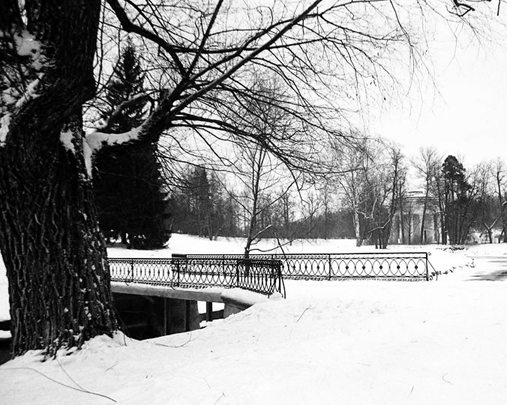
\includegraphics[width=0.45\textwidth]{thres/winter_o}}
\qquad
  \subfloat[Binary image obtained through thresholding]{\label{fig:thres1}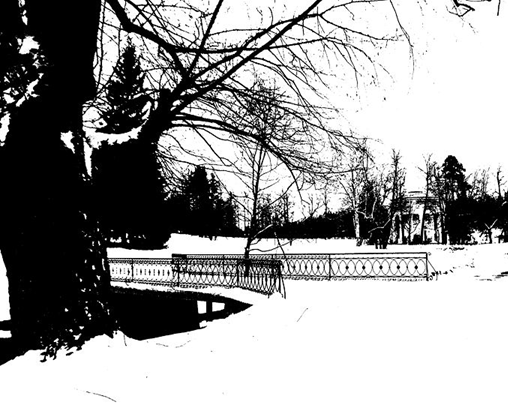
\includegraphics[width=0.45\textwidth]{thres/winter_thres}}
  \caption{Gray-scale Image before and after a thresholding effect is applied. Images taken from \cite{web:thresholding}}
  \label{fig:thres1}
\end{figure}

\section{Distance Transform}
\label{sec:dt}

A distance transform or distance map is a representation of a digital image
that is obtained by converting a digital binary image, consisting in object
and non-object pixels, to another image in which each pixel has a value
corresponding to the distance to the nearest non-object pixel. The object 
pixels can be considered as foreground and the non-object pixels as
background. The obtained image is then a sort of gray-scale representation
of the foreground pixels in the binary image.\\
The pixel mapping depends mainly on the distance metric, which is the 
measurement method of distance between image pixels. Different metrics have been 
studied to find distance maps such as 
\emph{City Block or Manhattan},
\emph{Chessboard}, \emph{Euclidean}, \emph{Chamfer 3-4}, \emph{Octagonal}, among
others.\cite[p.363]{dtresearch}. There exist a great amount of
distance metric of other kinds that are useful for different purposes.
These are commonly derived from the previous.
Fig.\ref{fig:dtexamples} shows the images obtained by applying different distance metrics.

\begin{figure}[h t b p ! H]
 \centering
   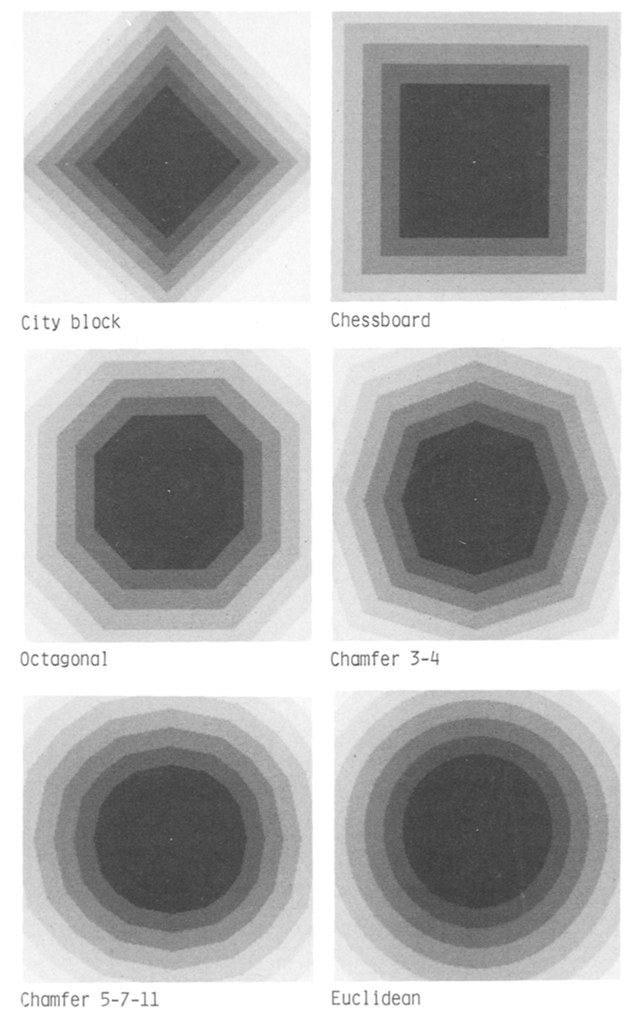
\includegraphics[scale=0.4]{dt/dtref}
 \caption{The distances from a point for the six distance transformations.
 The lighter the color the larger the distance \cite[p.365]{dtresearch}}
 \label{fig:dtexamples}
\end{figure}

As stated in \cite{dtresearch2} 
distance transforms play a central role in the comparison of binary images, 
particularly for images resulting from local feature detection techniques such 
as edge or corner detection. For example, both the Chamfer
and Hausdorff matching approaches make use of distance transforms in comparing binary images. 
Distance maps can also be interpreted as landscapes of islands 
where the label of every pixel indicates the height of the region. This allows
the detection of ridges and peaks which is a straightforward way to find the
skeleton of an object.\cite[237]{ridgedt}. The nature of distance transforms
in which the objects are represented as contour layers of different depth
makes them also a useful tool for edge analysis and to improve efficiency of 
morphology algorithms such as \emph{Thinning} and \emph{Thickening}.\\

\section{Skeletonization}
\label{sec:skeletonization}

A skeleton is a compact and simple representation of an object that consists of a thin
version of it that is equidistant to its boundaries and preserves many of
the topological and geometrical characteristics of the original image, as explained in
\cite{wikipedia:skeleton,ssm,augmented}. Usually the skeleton is defined as the centers
of maximal discs contained in the original image, \cite{ssm,augmented}.
Regardless of the definition that is adopted, if the skeleton points are attributed with their distances
to the original boundary of the object, the skeleton can be used to exactly 
reconstruct the original shape. Figure \ref{fig:genskeleton} shows a skeleton calculated
from a horse shape and the original binary image.\\

\begin{figure}[h t b p ! H]
  \centering
  \subfloat[Binary Image]{
\includegraphics[scale=0.8]{skeleton/horsebinary}}
\qquad
  \subfloat[Skeleton obtained using the ssm of the distance transform\cite{ssm}]{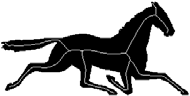
\includegraphics[scale=0.8]{skeleton/horseskeleton}}
  \caption{Horse binary shape and skeleton obtained using the ssm of the distance transform. Images taken from \cite{ssm}}
  \label{fig:genskeleton}
\end{figure}


Depending on the way they are produced, skeletons can be categorized in different types.
Telea et al describe three types in \cite{augmented}, such as: \emph{Morphological Thinning},
\emph{Geometric Methods} and \emph{Distance transform}. The \emph{Morphological Thinning} methods iteratively peel off (or reduce) the boundary, layer by layer, identifying
points whose removal does not affect the object's topology. These are usually 
straightforward and usually require intricate heuristics to ensure the skeletal
connectivity, as mentioned in \cite{augmented}. Two fast parallel approaches that
ensure connectivity using the \emph{Morphological thinning} method are described
in \cite{onepass} and \cite{thinning}.\\
The \emph{Geometric Methods} compute the Voronoi diagram of a discrete polyline-like
sampling of the boundary. A Voronoi diagram is the boundary's medial axis. ``Such 
methods produce an accurate connected skeleton, but are fairly complex to implement,
require a robust boundary discretization, and are computationally expensive''
\cite[p.251]{augmented}. The third defined method computes \emph{the distance transform}
(see Sec. \ref{sec:dt}) of the objects boundary. The common approach consists in
finding the ridge points and connecting them \cite{maxima,euclideancentre,ridgedt}.
 Usually they can ensure the accurate localization of skeleton points 
but neither connectivity nor completeness.\\

Skeletons are important for object representation and recognition in different areas,
such as: computer vision, image analysis, and digital image processing, 
including optical character recognition, fingerprint recognition, visual inspection,
pattern recognition, binary image compression, and protein folding \cite{skprotein}.


\section{Shape Matching}
\label{sec:shapefitting}

Shape matching is a central problem in visual information systems,
computer vision, pattern recognition and robotics \cite{matchingbook}. 
It consists of identifying the area or contour of a specific
shape or class of shapes in an image, and plays a fundamental
role in content extraction from images and content-based image
retrieval. In \cite{matching2} Veltkamp explains that shape 
matching deals with transforming a shape and measuring the 
resemblance with another one, using some similarity measure, that 
normally correspond to the notion of distance between shapes.\\
The concept of shape is abstract, but most approaches in 
shape matching represent a shape as a geometrical object.
This can be both a set of points, curves, surfaces, solids etc.
and a geometrical pattern modulo some transformation group,
in particular similarity transformations (translations, rotations 
and scalings), as is stated in \cite{matching2}. Usually a
geometrical pattern of a shape called shape descriptor
is used to represent the class of the matching object. There are
different types of shape descriptors depending on the information
they supply and the nature of the problem (see Sec.\ref{sec:shapedesc}) \\

There are different studied ways to approach the shape matching 
problem. The emphasis on this section will be on the Computational
Geometry based approaches for shape matching, since is the most related with
the approach followed in this thesis work. Computational
Geometry studies algorithms that can be declared in terms of 
geometry.\\

In \cite{matchingbook} Veltkamp and Hagedoorn mention different 
approaches of shape matching such as: tree pruning, the
generalized Hough transform or pose clustering, geometric hashing,
the alignment method, statistics, deformable templates, relaxation
labeling, Fourier descriptors, wavelet transform, curvature
scale space and neural networks.
They also categorize the matching techniques in two main groups:
\emph{global image transforms} and \emph{global objects methods}.
The \emph{global image transform} group refers to the techniques that
``transform the image from color information in the spatial
domain to color variation in the frequency domain''. 
These approaches do not represent the shape explicitly for 
matching, instead they represent color or intensity transitions 
in the image. This makes impossible to measure the difference of 
two images in terms of shape as well as match a shape with a 
specific part of an image.\\
On the other hand the \emph{global object methods} work with a complete
object area or contour and can analyze specific areas in the 
image instead of requiring to process the whole image as in 
the global image transforms. In order to perform a proper
matching, the objects in the image have to be completely and
clearly segmented. Some of these methods are: \emph{moments}, where an
object is described as a set of moments, \emph{modal matching},
where the boundary is used instead of the area and is described 
with Fourier descriptors and \emph{curvature scale space}, where a
scale space and parameterized representation of the contour of the 
objects is used.\\

Veltkamp describes in \cite{matching2} four different forms in
which shape matching is studied, given two shape patterns
and a dissimilarity measure. These are:

\begin{itemize}
\item \textbf{Computation Problem: }Compute the dissimilarity
  between the two patterns
\item \textbf{Decision Problem: }For a given threshold, decide
  whether the dissimilarity is smaller than the threshold
\item \textbf{Decision Problem: }For a given threshold, decide
  whether there exists a transformation such that the
dissimilarity between the transformed pattern and the other 
pattern is smaller than the threshold
\item \textbf{Optimization Problem: }Find the transformation
that minimizes the dissimilarity between the transformed
pattern and the other pattern.
\end{itemize}

A well studied optimization approach for shape matching is
Active Contour Models (\emph{Snakes}),  which inspired much 
of the shape fitting approach of this work 
(see Sec \ref{sec:metfit}). In \cite{snakes} a snake is defined 
as an energy-minimizing spline guided by external constraint
forces and influenced by image forces that pull it toward 
features such as lines and edges. The \emph{snakes} are said to
be active contour models because they lock onto nearby edges,
localizing them accurately.\\
The \emph{snakes} model is defined as a controlled continuous spline that is bound
by internal and external image forces, called energies. The external energy models how well
the deformed model matches the data. The internal energy models
the objects resistance to be pushed by the external force into directions not coherent
with the prior knowledge \cite{deformable}. In this case, the internal energy  imposes 
a ``piecewise smoothness constraint'' \cite{snakes}. This means that a contour is
pushed to an image feature by the external force while the contour itself exhibits resistance
to be deformed into a non-smooth curve. As is explained in \cite{deformable} the image forces push the snake toward
salient image features like line, edges and subjective contours, while the external constraint forces
are responsible for putting the snake near the desired local minimum.\\

Given these definitions, let $M$ be the model and $D$ a data set, 
the total energy $E$ can be defined as:

$$E(M) = E_{ext}(M,D) + E_{int}(M)$$

where $E_{ext}$ is the external energy function and $E_{int}$ the 
internal energy function. 
Having this, the optimization algorithm consists of minimizing the objective
function until the best solution is found.


\section{Shape descriptor}
\label{sec:shapedesc}

A shape descriptor is a structured abstraction of a class
of shapes that describes them in geometrical terms.
Shape descriptors can have either fixed or variable
geometrical shape. Variable descriptors depend on the different values assigned to its
parameters, different shapes are generated but still belong to the same type or class of shapes.
Shape models have been used widely to achieve robust interpretation of complex
images \cite{wormparam}. They allow image evidence to be organized into plausible interpretations
which can then be verified.\\

Latecki et al divide shape descriptors into three
main categories: \cite{shapenonrigid}
\begin{itemize}
\item \textbf{Contour based descriptors: }The contour of a given object is 
mapped to some representation from which a shape descriptor is derived
\item \textbf{Image based descriptors: }The computation of a shape descriptor
is based on summing up pixel vales in a digital image containing the silhouette
of a given object; the shape descriptor is a vector of a certain number of
parameters derived this way
\item \textbf{Skeleton based descriptors: }After a skeleton is computed, it is
mapped to a tree structure that forms the shape descriptor; the shape similarity
is computed by some tree-matching algorithm 
\end{itemize}

Considering that basically shape descriptors are ``attempts to quantify shape in 
ways that agree with human intuition''\cite[p.1]{desclecture}, any kind of 
geometrical interpretation that covers the contents or properties that want 
to be described on a shape, can be used as a shape descriptor.
In \cite{desclecture} region-based shape descriptors are covered which are such
that attempt to describe a shape based on the geometrical and numerical properties
of the region of the shape. Some simple descriptors are mentioned such as:
area, perimeter, (Non-)Compactness or (Non-)Circularity, Eccentricity, Elongation,
Rectangularity and Orientation. Any combination of this properties of a shape are
useful to describe them in a basic and general way.
Other more complex properties are mentioned to improve the accuracy of the 
descriptor: \emph{convex hull}, \emph{extremal points}, \emph{profiles},
\emph{ moments} and \emph{profile moments}. \emph{Convex hull or bays} 
describes the shape by measuring the number or size of concavities in the 
shape. \emph{Extremal points} is based on finding the points that
are at the extreme of the shape. This can be a simple representation as the 
\emph{bounding box} or a more powerful one as it is finding the eight extremal
points defined by: top left, top right, left top, left bottom, bottom right,
bottom left,right top and right bottom. \emph{Profiles} shape descriptor 
is based on the number of pixels that the shape has in a given direction:
 either vertical, horizontal or diagonal. \emph{Moments} refer to the
 calculation of \emph{moment} statistical properties and 
\emph{profile moments}, or a combination of the last two.\\
\cite{web:wikishape} classifies shape descriptors by their
invariance with respect to the transformations allowed in the associated
shape definition. The main classes are descriptors invariant with respect 
to congruency and invariance with respect to isometry. The congruency class
comprehends indentical shape descriptors for congruent shapes 
(shapes obtained from
translation, rotation or mirroring). The intrinsic shape descriptor refer
to those that do not change with different isometric embeddings of the shape,
and thus can be applied accurately to deformable objects.

Depending on the properties that are controlled and measured, the descriptor
may or may not allow to reconstruct a shape of the class. In \cite{wormparam} 
a trainable method of shape representation is described which can
automatically capture the invariant properties of a class of shapes and 
provide a compact parametric description of variability. The method was
applied on worms, obtaining a shape descriptor that reconstruct different
bending worm shapes by modifying the values of the parameters.\\

\section{Splines}
\label{sec:splines}

The term spline, as it is used in this work, refers to a piecewise polynomial curve. Splines
are wide used in computer science subfields because of the simplicity of their constructions,
their easy and accuracy of evaluation, and their capacity to approximate complex shapes
through curve fitting and interactive curve design, as mentioned in \cite{web:splines}.
The continous signal representation is particularly apposite for 
problems such as: edge detection, surface fitting and multiresolution
techniques. It is useful for many other problems in computer
vision such as: optical flow, surface reconstructoin, the recovery
of lightness and color, shape from shading and stereo matching,
\cite[821]{splinespap}.

Special types of splines receive different names, depending of different conditions.\\
A commongly used type of spline in object recognition is the Hermite spline.This is
is a third-degreee spline, expressed using Hermite polynomials to represent each of the 
individual polynomial pieces. 
Several methods have been invented to fit such splines to given data points such
as \emph{Cardinal Splines, Catmull-Rom splines, Kochanek-Bartels splines}. They allow to
construct smooth curves that go through every point in a given data set. Thus, \emph{e.g.} 
given a series of points belonging to the contour of an object, a smooth shape can be 
calculated that models the shape of the defined object.  
Such as B-splines, Hermit splines have a number of advantages for image processing, as
mentioned in \cite{splinespap}.
First, they are usually smooth and well behaved, therefore the do not tend to oscillate
as higher order polynomials do. Second, the juxtaposition of local polynomial approximations
may produce strong discontinuities in the connecting regions, B-spline
surfaces, by contrast, are continous everywhere. 
Finally, they can be evaluated efficiently.
%\cleardoublepage  
\chapter{Methodology}
\label{chap:methodology}

\section{Development Methodology}
\label{sec:devmet}

\section{Solution Methodology Design}
\label{sec:solmet}

This sections presents the solution methodology which consists in the different
steps in image processing that must be performed in order to successfully fit the shape of 
\emph{C.elegans} worms present in digital images. First a general description
of the solution is presented where the shape fitting approach is explained, indicating
the different processes involved in the solution design. Then for each process 
a reasoning of its requirement and usefulness is given, as well as 
the corresponding 
implementation approach.

\subsection{Previous reasoning}
\label{sec:reasoning}

As stated in \cite{binaryshape} and also covered in
\cite{deformable,matching2,matchingbook} shape 
matching is usually accomplished adopting a shape
descriptor and then placing a constructed shape sufficiently 
close to the image shape and adjusting the values of 
the parameters of the descriptor until a match is found.
A shape descriptor is a representation of a 
specific class of objects that is defined in geometrical
terms. It is comprised of a number of parameters, where 
different values for each parameter give different 
shapes of a given class of objects.
This approach is appropriate when the objects
that are to be matched can be categorized in a certain 
class and thus can be represented or described in terms
of geometry, \emph{i.e.} a shape descriptor.\\

The problem of study aims the detection of worms,
particularly those belonging to the \emph{C.elegans} species. Given
the vermiform (worm shape) property of these individuals,
the objects to detect can be defined as part of a 
\emph{worm} class,
that would refer geometrically to long, thin and cylindrical 
shapes, in 
general terms. Following this idea, a shape descriptor could be
designed that comprehends a cylindrical, long and connected
shape, with two endpoints and different thickness along a medial
axis. Then the problem would be reduced to find every pair of
endpoints belonging to each worm in the image, place an approximated
shape (built through the shape descriptor) near the matching worm,
and adjust the values of the parameters of the shape descriptor until
a acceptable match is found.\\

To design a methodology for the solution of the problem the following
points must be taken into consideration: the nature of the input
images, the positional identification of worms in the global image,
the gathering and loss of information and the efficacy and efficiency
of each of the involved processes (and their respective algorithms).
For this study the input images consist of a number of worms that
are put together in liquid media. The image can contain some noise such as
shadows, water bubbles or little remains that do not belong to the worms, so
these last, as objects of study, must be separated from the rest of 
the information in the image. The position of each individual
worm in the image is variable and can be distinguished into two 
groups: \emph{worm clusters} and \emph{isolated worms}. A 
\emph{worm cluster} corresponds to a group of worms in which 
each worm is connected to any other directly or indirectly
through overlapping. It can also be described as a group of worms in which a 
path can be traced from every worm to another without passing over 
background pixels. On the other hand, an \emph{isolated worm} is such
that it is surrounded by background pixels and does not overlap
with any other worm. The image can be segmented by separating the different 
\emph{worm clusters} and \emph{isolated worms}, so each segment
can be processed individually. The contour of \emph{isolated worms} can be
traced automatically following the pixels that are closest to background pixels.
These can also be used to generate a profile that will set the general values
for the shape descriptor that best represents the shape of the worms in the image.
The worms that are clustered can be matched through an energy minimization
process, based on the manipulation of the shape descriptor and its distance
to the matching image, in order to obtain the best possible match.

\subsection{Methodology description}
\label{met:description}

Following the previous reasoning, a methodology was designed taking into account
the main components of the matching process, as reasoned before, such as: 
determination of the objects 
of study, objects segmentation, worm shape descriptor and matching based on 
energy minimization.
Below the solution methodology is described, pointing out the sequential steps
that are followed to match and fit the shape of every worm in the input image.
In Fig. \ref{fig:methsol}, a graphical description of the solution methodology is
presented.\\

\begin{figure}[h t b p ! H]
 \centering
   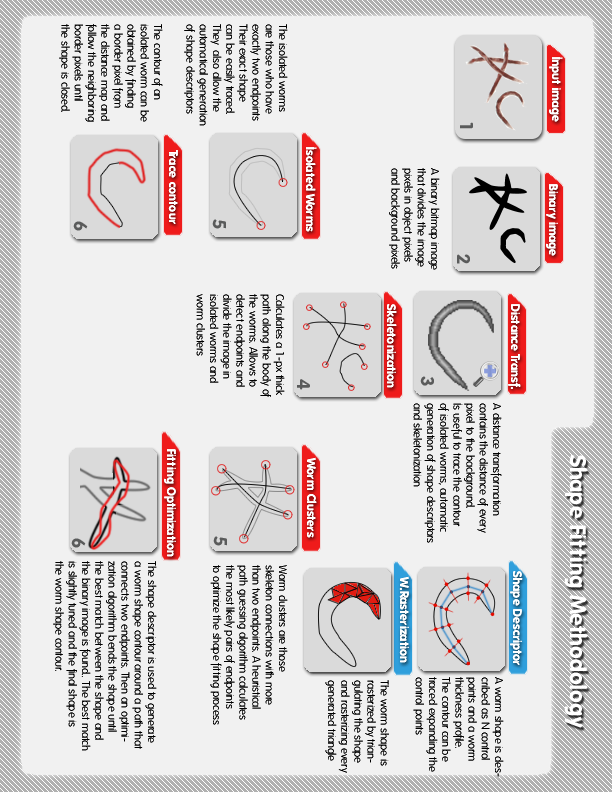
\includegraphics[scale=0.75]{diagrams/design-methodology.png}
 \caption{Graphical description of the solution methodology for the shape detection
 of \emph{C.elegans} worms in digital images}
\label{fig:methsol}
\end{figure}

Given the input image, the first step is to separate the pixels belonging to the object
of study from the rest of the image pixels. A thresholding algorithm is then used to
obtain a binary image that separates worm pixels from background pixels. Usually some
noise is obtained after the thresholding process, but it is ignored in further processing.
This corresponds to an initial segmentation of the input. Once one have a binary image, a
distance map can be obtained in which each pixel represents the distance to the 
nearest background pixel, as explained in \cite{dtresearch}. The distance transformation
makes possible to identify the contour pixels in the binary image, which makes it a fundamental
tool for the automatic generation of a shape descriptor, contour tracing on isolated worms 
and optimization of the skeletonization algorithm, among others. Having the image 
separated in object pixels and background pixels, the image can be segmented to separate
the worms. \\

The image worms have been distinguished into two groups: \emph{isolated worms}
and \emph{worm clusters} (see Sec.\ref{sec:reasoning}). A way to differentiate the image worms
is to count the number of endpoints of every object (as defined after the binary transform).
An object with exactly two endpoints would correspond to an \emph{isolated worm} while
more than two points indicate the presence of overlapping worms, thus a \emph{worm cluster}.
At the same time a path from one endpoint of a worm to another is needed to match
the shape, due to the need of placing the matcher shape near to the matching shape, which
is a usual approach for shape matching, as covered in Sec. \ref{sec:shapefitting} and
Sec. \ref{sec:reasoning}. Having said this, a process of skeletonization would provide a simple
way to recognize endpoints as well as an approximated connected medial path between the
endpoints of the image objects. After this process, the image will be segmented into 
many different subareas of the images corresponding to both clusters and \emph{isolated
worms}. Each type of worm group is processed in a different way in order to match
the shape.\\

\subsubsection*{Isolated Worms}
The \emph{isolated worms} shape contour can be traced easily by selecting a border pixel
(indicated in the distance map) and following the neighboring contour pixels until the
initial pixel is reached back again. Then the whole shape can be rasterized by 
triangulating it through the \emph{ear clipping triangulation method} and then rasterizing
each triangle separately.This provides all the pixels belonging to the shape, 
\emph{i.e.} a match.
The nearly perfect match that can be obtained from the \emph{isolated worms} makes 
possible to calculate a worm profile from the currently analyzed worms in order to
generate an accurate shape descriptor (this is explained thoroughly in 
Sec. \ref{sec:metshapedescriptor}).

\subsubsection*{Worm Cluster}
To match the shape of the worms present in a \emph{worm cluster}, first the number of worms in the cluster is determined (follows from the number of
endpoints), then the best match between pairs of endpoints is found. Given a pair of 
endpoints, the path between them is calculated and then a matcher worm shape is generated
from the shape descriptor, selecting a given number of control points in the path.
Then an energy minimization process is performed that varies the angles between the 
straight lines that connect the control points (generating different shape representations),
until the best match is found. Finally the contour of the shape descriptor is slightly 
modified by finding the closest contour segments (or a lower value in the distance map)
to the contour points, in order to adapt the generic shape silhouette to 
the matching object. 

This process can be repeated between every pair of endpoints and then the best match is chosen.
On the other hand a path guessing algorithm
can be used to find the most likely path between endpoints, \emph{i.e.} the path from
one point to another in the cluster skeleton that most likely belongs to a worm 
(see. \ref{pathguessing}), in order to avoid the cost of trying every pair of endpoints. Since the total energy is
the sum of energies of each worm, speed can be improved further by branch and bound.\\

In the following sections, each of the subprocesses involved in the solution
methodology are explained, covering their need and usefulness as
well as the followed implementation approach.

% ADD THE MANUAL MODIFICATION OF THE RESULTS
  

\subsection{Thresholding}
\label{sec:metthres}

Since the main purpose of this study is to fit the shape of \emph{C.elegans} worms on digital
images, it is useful to differentiate these from the rest of the image in order to perform a more 
accurate analysis. The shape of the worms
can be characterized as objects and the rest of the image as background. More precisely
the image pixels can be separated into two groups: object pixels, that are all of those
that belong to a worm shape and background pixels, that are all the remaining ones.\\

Given this theoretical characterization, a thresholding filter would come to be a useful tool 
to locate the objects of study in the digital representation and to discard unnecessary 
information, obtaining a binary image from the original one. A binary image would then provide
an initial segmentation of the processed image, being as well a key element to obtain
a distance transformation, as explained in Sec. \ref{sec:metdt}.

\subsubsection{Implementation}
\label{sec:thresimp}
There are four thresholding filters for 2D images implemented on \emph{Endrov}, these are: 
\emph{Fukunaga}, \emph{Max entropy}, \emph{Otsu} and \emph{Percentile}, that cover the 
histogram and entropy-based thresholding methods categories as defined in Sec.\ref{sec:thresholding}.
Considering that the implemented methods are sufficiently different and given the transparency
of \emph{C.elegans} worms, it is hard to determine theoretically which would be the most appropriate 
thresholding method to obtain an accurate binary image from the study data-set. In order 
to select a thresholding method a series of experiments where performed tweaking the parameters
for the different mentioned methods, as explained on Sec.\ref{exp:thres}.
The selected method was \emph{Percentile Threshold 2D} with a percentile value oscillating from
$0.072$ to $0.11$ on the different test images.\\

Figure \ref{fig:wormthres} shows a binary image obtained after applying
the \emph{Percentile Threshold 2D} method with a percentile value of $0.074$

\begin{figure}[h t b p ! H]
  \centering
  \subfloat[Original image]{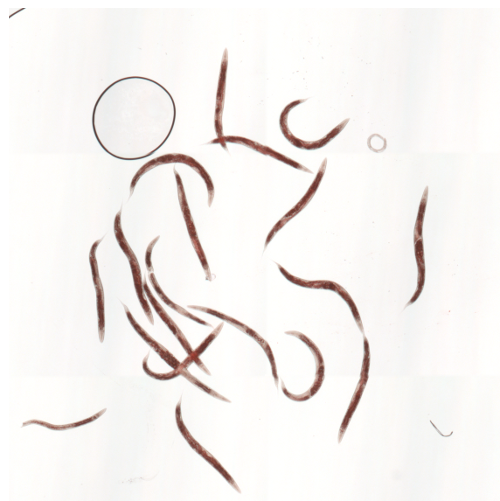
\includegraphics[width=0.45\textwidth]{original.png}}
\qquad
  \subfloat[Percentile Threshold. Value=0.074]{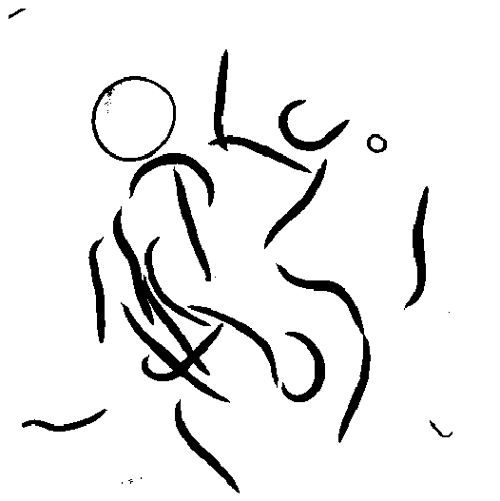
\includegraphics[width=0.45\textwidth]{thres/worms}}
\caption{Worms in liquid media. Original image and binary image obtained through
Percentile Thresholding with a percentile value of 0.074}
  \label{fig:wormthres}
\end{figure}

\subsection{Distance transformation}
\label{sec:metdt}

In this shape fitting approach for \emph{C.elegans} worms the distance transformation
of the given image is used thoroughly for contour detection and different kinds of image 
segmentation procedures. Specifically the distance map allows to detect and follow
the exact contour of isolated worms (Sec. \ref{sec:metiso}), 
is useful in the shape profile generation (Sec. \ref{sec:metwormprof}), and essential in the heuristic
guessing of the more likely worm-paths in \emph{worm clusters} (Sec. \ref{sec:metcluster}).
It also improves the performance of the iterative thinning algorithm designed by 
\emph{Zhang and Suen} \cite{thinning} as it is described on Sec. \ref{sec:metsk}

\subsubsection{Implementation}
\label{sec:dtimp}

 As stated in \cite[p.196]{fastdt} the algorithms of distance transformation can be categorized into two classes: one is the iterative 
 method which is efficient in a cellular array computer since all the pixels at each iteration can be processed in parallel, and the other 
is sequential (or recursive) method which is suited for a conventional computer by
 avoiding iterations to be independent of object size. 
Using the general machines that most people working in digital image processing
 have access to, sequential algorithms are often much more efficient than
 iterative ones. For this reason a sequential approach was chosen to calculate the
distance transformation of the input images. Particularly the two-scans transformation
using 3x3 neighborhoods \cite{fastdt} which is both efficient and easy to implement.\\

In the mentioned paper a distance map calculation algorithm is described which consist
of only two scans of the image bitmap, one left to right - top to bottom, and another
right to left - bottom to top, with one operation per pixel. This makes the complexity
of the algorithm $\mathcal{O}(N)$ where $N$ is the size of the image array.
In \cite[p.197]{fastdt} a pseudo-code for \emph{Chessboard} and 
\emph{Manhattan or city-block} distances is given, while in \cite[p.198]{fastdt} the 
definition is extended to improve the efficiency of the calculations needed to 
generate a distance map using \emph{Euclidean} distances.
The two-scans algorithm was implemented using the three different distance metrics
mentioned before. This allows a wider analysis on the behavior and accuracy of the shape 
fitting process from one metric to another,``The city block or chessboard distance
measures are sensitive to the rotations of an object, but the Euclidean distance
measure is rotation invariant. However, its square root operation is costly...''
\cite[p.332]{eucskeleton}. Given the straight-like shape of worms and the different levels
of accuracy of the distance metrics it is hard to tell at first sight which would be 
the most adequate to use, so it had to be determined experimentally, as explained in \ref{exp:dt}.
The figure \ref{fig:distance} shows the binary image and three distance maps obtained 
from a single worm image.

\begin{figure}[h t b p ! H]
  \centering
  \subfloat[Binary Image]{\label{fig:manh}
\includegraphics[width=0.45\textwidth]{dt/binary}}
\qquad
  \subfloat[Manhattan metric]{\label{fig:manh}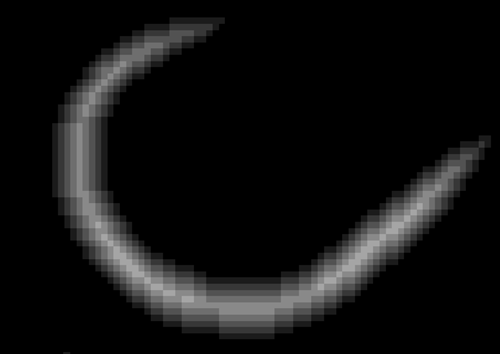
\includegraphics[width=0.45\textwidth]{dt/manhattandt}}
\qquad                
  \subfloat[Chessboard metric]{\label{fig:chess}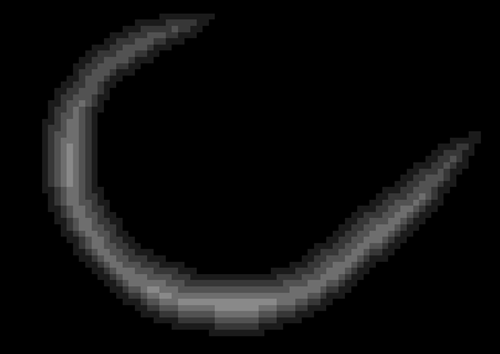
\includegraphics[width=0.45\textwidth]{dt/chessboarddt}}
\qquad
  \subfloat[Euclidean metric]{\label{fig:mouse}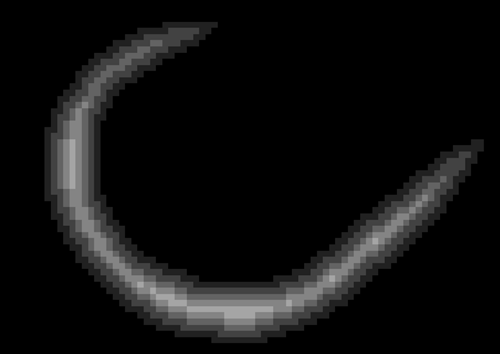
\includegraphics[width=0.45\textwidth]{dt/euclideandt}}
  \caption{Binary Image and Three Distance Transformation metrics from a single worm image}
  \label{fig:distance}
\end{figure}


\subsection{Worm Skeletonization}
\label{sec:metsk}

The skeletonization of the image corresponds to the process of obtaining a 
connected and thin (1-pixel width) medial axis that represents the worms in the 
image. This is a key process on the shape matching
approach followed in this work, as first mentioned on Sec. \ref{met:description}.
It allows to identify the amount of worms in the input image, to separate them 
distinguishing between \emph{isolated worms} and \emph{worm clusters}, and to
obtain an approximated path between endpoints 
of worms (that tends to the medial axis), which is the main element of the 
matching optimization process (see Sec.\ref{sec:metsegmentation}). The skeleton
image would be then fundamental to determine the area of the image in which
the worms are located and give estimated paths along which the different
worms would be disposed. \\

\subsubsection{Implementation}
\label{sec:skeletonimp}

For the purpose of this work the skeletonization algorithm to be selected must
ensure the connectivity of the skeleton points, \emph{i.e.} every skeleton point
must be connected to at least another skeleton point belonging to the same
skeleton. Also the skeleton connection must not be thicker than 1-pixel, this means that
when tracing a sequential path in the skeleton and being situated in a given skeleton 
point there must be only one neighbor skeleton point that can be selected to continue
the path direction, while remaining on the track of the skeleton of the same worm.\\

Provided that a distance map have been already calculated when the skeletonization 
process is carried out, an efficient approach would be to use a distance transform
based technique. Different methods consisting in finding ridge points on the distance
maps and then connect them have been covered in \cite{maxima,euclideancentre,ridgeineuc}.
The approach in \cite{maxima} was followed as a first attempt to calculate a thin
skeleton with a low time cost. This algorithm defines the ridge points as such pixels
that have the greatest numerical value among its 3x3 neighborhood (bitmap image) in the 
distance map. After finding the ridge points a \emph{up-hill} reconnection is performed, 
followed by a \emph{down-hill} connection for missing points. The study covered in \cite{maxima}
states that this approach allows to find successfully a connected 1-pixel-thin skeleton,
which was actually the case for \emph{isolated worms} or those which do not
overlap with other worms. Nevertheless for \emph{worm clusters} the obtained skeletons
were usually disconnected, thicker than 1-pixel and not accurate. Although the approach
seemed appropriate in theory, the costful reconnecting operations and the inaccurate
skeletons obtained for \emph{worm clusters} gave rise to the need for a different
approach.\\

Given the long, thin and cylindrical shape of the worms in general, a thinning algorithm
approach that reduces the different layers by removing pixels that should not 
belong to the skeleton was then taken into account. In \cite{thinning} an iterative and 
parallel thinning algorithm is presented, that consist in two sub-iterations per main 
iteration aimed at deleting the south-east boundary points and north-west boundary points 
respectively. The study is aimed at parallel computers so the different operations
in each pixel can be performed at the same time, improving the performance. In order
to avoid the requirement of using a parallel computer without losing the time performance 
improvement, the distance map was used to discard unnecessary pixel checking (those
belonging to inner layers). Thus in each iteration only the pixels belonging to the
currently selected shape layer are taking into account. The layers are defined by the
distance map value of its pixels. The first layer corresponds to a distance value
of one ($1$), the next to a distance value of two ($2$) and so on. This is presented in
algorithm \ref{thinninalg}.\\

\begin{algorithm}                     
\caption{Calculate shape skeleton}         
\label{thinninalg}                    
\begin{algorithmic}                   
\STATE $shapePts \leftarrow getBinaryObjectPixels()$
\STATE $dtImage \leftarrow getImageDistanceMap()$
\STATE $contourIndex \leftarrow 1$
\STATE $makeThinner = True$

\WHILE{$makeThinner$}

\STATE \COMMENT{remove south-east boundary points and the north-west 
corner point}
\FOR{$pixel$ in $shapePts$}
\IF{$dtImage(pixel) > contourIndex$}
\STATE \COMMENT{skip iteration}
\ELSE
\STATE $pixelRemove \leftarrow southEastCondition(pixel)$
\IF{$pixelRemove$}
\STATE $shapePts.remove(pixel)$
\STATE $makeThinner \leftarrow True$
\ENDIF

\ENDIF
\ENDFOR

\STATE \COMMENT{remove the north-west boundary points and the
		south-east corner points}
\FOR{$pixel$ in $shapePts$}
\IF{$dtImage(pixel) > contourIndex$}
\STATE \COMMENT{skip iteration}
\ELSE
\STATE $pixelRemove \leftarrow northWestCondition(pixel)$
\IF{$pixelRemove$}
\STATE $shapePts.remove(pixel)$
\STATE $makeThinner \leftarrow True$
\ENDIF
\ENDIF
\ENDFOR
\ENDWHILE
\STATE 
\RETURN{$shapePts$}

\end{algorithmic}
\end{algorithm}

The algorithm deals well with overlaping worms by constructing a path that is very close
from the shapes medial axis, and results in a totally connected 1-pixel width skeleton.
In fig. \ref{fig:skeleton} the skeleton of a sample image is shown. Every worm in the 
image that was previously identified in the binary image obtaining process 
(see \ref{sec:metthres}) is successfully \emph{skeletonized}.

\begin{figure}[h t b p ! H]
 \centering
   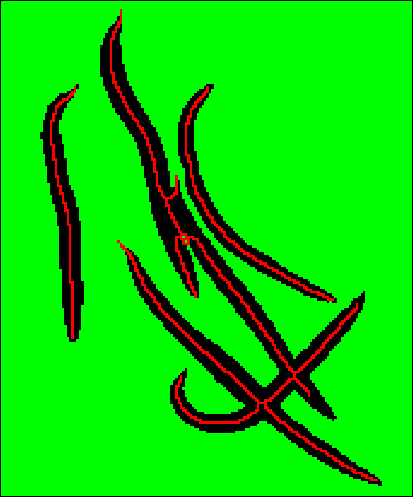
\includegraphics[scale=0.75]{skeleton/skeleton.png}
 \caption{Skeleton obtained through iterative thinning over a worm binary image}
\label{fig:skeleton}
\end{figure} 


\subsection{Worm Segmentation}
\label{sec:metsegmentation}

%why segmentation. What would be obtained
Since the goal is to match the shape of individual worms,
it is necessary to locate them in the image and then separate them 
as much as possible, \emph{i.e.} to segment the image (see Sec. \ref{sec:segmentation}). 
This allows to improve the efficiency and accuracy of the 
shape fitting process, while reducing the matching area and thus the amount of 
different combinations that must be taken into account. After the process of 
\emph{skeletonization} a set of paths are obtained 
between endpoints of worms (the objects of study), in some cases overlapping. 
By identifying the worm endpoints and tracing the paths that connect them together,
the different groups of paths can be separated, thus segmenting the image.
As explained in Sec. \ref{sec:metsk} and Sec. \ref{sec:reasoning}, the different groups
of paths can be distinguished, in correspondence to the objects they represent,
by \emph{isolated worms} and \emph{worm clusters}. Then the shape fitting process
of the whole image would consist of matching and fitting the worms present in each of
the obtained sub-images separately.\\

Another process of segmentation that is performed is the identification of single
worms paths, in both \emph{isolated} and \emph{cluster} worms. For \emph{isolated worms}
the path that determines its medial axis is used, first to find the surrounding contour to
fit its shape (see Sec. \ref{sec:metiso}), and second to generate a profile that 
would define a general representation of the worms in the image through a shape
descriptor, as is explained in Sec. \ref{sec:metwormprof}.
On the other hand, for \emph{worm clusters}, correct worm paths must be found between endpoints that
permit the construction of a general shape, in order to determine if a worm can be matched
between those two endpoints through the matching optimization process. These paths are chosen
among all the technically possible paths between endpoints, or by
a more sophisticated path guessing algorithm that will be described below in the
implementation section.
%think above begs for some reformulation. shorter sentences!



\subsubsection{Implementation}
\label{segmentimp}


\subsubsection*{Worm Endpoints}
\label{sec:wend}
The skeleton calculation returns an image 
containing 1-pixel-width groups of curves or paths, which means that each pixel 
is a neighbor of either one or two other pixels. The pixels that are connected with 
two other pixels (two neighbors) are \emph{body-pixels}, which belong 
to the path and are not endpoints. On the other hand those that are connected with 
only one other pixel are endpoints, thus each one could belong to the extreme of a
worm. It is important to consider that since the thinning algorithm used to obtain
the skeleton (covered in Sec. \ref{sec:skeletonimp}) consists in removing the shape
layers until finding pixels that are not surrounded, the endpoints found in the
skeleton will not necessarily correspond to worm endpoints.\\

In order to find the pixels that are actually worm endpoints a skeleton expanding process
is performed that aims to stretch the skeleton path up to a contour point that 
would come to be the worm endpoint. The skeleton expanding algorithm uses the definition
of \emph{directional neighborhood} stated in \cite[p.334]{maxima}, where given 
a pixel $P$ in the bitmap, a \emph{directional neighborhood} $D$ of $P$ is 
conformed by those pixels that belong to the \emph{8-neighborhood} of $P$ and that
are located within $\pm$ $45^{\circ}$ slope changes from the current medial axis 
orientation of $P$. In fig. \ref{fig:directional} three examples of directional
neighbors are presented. The algorithm consist in following the best directional path
starting in every endpoint and expanding the skeleton until a contour pixel is found.
 
\begin{figure}[h t b p ! H]
 \centering
   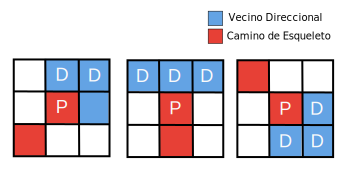
\includegraphics[scale=1]{skeleton/directional}
 \caption{Three different directional neighborhoods}
 \label{fig:directional}
\end{figure}

The expanding algorithm can be summarized in the following steps:
\begin{itemize}
\item Select an endpoint
\item Find the previous skeleton point and calculate the directional neighborhood
\item Select the directional neighbor with the lowest distance transformation pixel,
  and mark it as skeleton pixel.
\item If the neighbor is not a contour point repeat the process.
\end{itemize}

A filtering process is done to remove incorrect object pixels, that consists in
removing sub-skeletons that have a size (number of pixels) lower than a small 
threshold. This allows to remove some slightly noisy regions and incorrect endpoints.
Once the skeleton is successfully expanded, the endpoints of the skeleton are considered
worm endpoints. 
It must also be considered that some worm endpoints cannot be detected following this 
process, particularly in crowded images where there is a big chance that the
overlaps ``hide'' the endpoints. This is considered when selecting paths between 
endpoints, as explained in Sec. \ref{sec:pathguessing}.


% ADD THE MANUAL ADDITION OF ENDPOINTS

\subsubsection*{Group segmentation}

Having detected every worm endpoint, the image can be segmented by determining
the endpoints that are bound together through a skeleton path, \emph{i.e.} finding 
the different \emph{isolated worms} and \emph{worm clusters}.
As previously explained, the overlapping worms in the image are bound together
as one object in the binary image obtaining process, so then in the skeletonization
process the endpoints belonging to \emph{worm clusters} are bound together as well,
through a skeleton path.
Based on the previous reasoning an algorithm was designed that detects the endpoints 
that are bound together through the path that links them, separating the 
linked paths into different groups. Those paths that link together exactly two
endpoints represent \emph{isolated worms} while a different number of endpoints
correspond to \emph{worm clusters}.
This method is described in algorithm \ref{groupsegment}. The algorithm consist of
basically following every different
possible path starting on an endpoint until all the endpoints of a group have been 
reached. 

\begin{algorithm}                     
\caption{Calculate shape skeleton}         
\label{groupsegment}                    
\begin{algorithmic}                   

\STATE $endPtList \leftarrow$ list of endpoints
\STATE $clusterIndex \leftarrow$ 0
\FOR{$endpoint$ in $endPtList$}
\IF{$endpoint.wasVisited()$}
\STATE \COMMENT{skip iteration}
\ELSE
\STATE $clusterIndex +=1$
\STATE $followPath(endpoint,clusterIndex)$
\ENDIF
\ENDFOR
\end{algorithmic}
\end{algorithm}

\begin{algorithm}                     
\caption{Follow Path algorithm ( $followPath(currentPoint,clusterCount)$ )}         
\begin{algorithmic}                   

\REQUIRE $currentPoint$
\REQUIRE $clusterCounter$

\IF{not $currentPoint.isSkeletonPoint()$}
\RETURN 
\ELSE
\STATE $addToCluster(endpoint,clusterIndex)$
\ENDIF

\STATE \COMMENT{continue tracing path}
\IF{$currentPoint.isEndPoint()$}
\STATE $markEndPointAsVisited(currentPoint)$
\ENDIF
\STATE $neighbors \leftarrow getNeighborhood()$
\FOR{$n$ in $neighbors$}
\STATE $followPath(endPoint,clusterCounter)$
\ENDFOR

\end{algorithmic}
\end{algorithm}


\subsubsection*{Path guessing}
\label{sec:pathguessing}

The \emph{worm clusters} found through segmentation are defined by a set of endpoints
that are all connected through \emph{skeleton} paths, however the pair of endpoints
belonging to each worm in the image and an accurate skeleton path that
connects them is still unknown. The optimization algorithm, covered in \ref{sec:metfit},
performs a shape manipulation process to match the worms in the image given two endpoints
and the path that connects them. When the right skeleton paths are unknown the algorithm
tries every possible combination returning the best match as possible, with the 
consequent overhead in performance time . In order to improve the time efficiency of the 
algorithm as well as the accuracy of the matching (particularly avoiding incorrect
endpoints bounding), a path guessing algorithm was designed that performs a heuristic
guessing of the most-likely path between endpoints.\\

The algorithm is based in the idea of avoiding paths that continue unnatural conformations
of the worms shape. This means that given $S$ last steps in the skeleton tracing, the
next step $S+1$ will tend to follow the direction that was being followed, thus
avoiding unnatural bendings or abrupt changes in the shape. An important issue when 
following the most common direction in the last $S$ steps is that in some cases
the path tracing will tend to avoid \emph{path bifurcations}. 
A \emph{path bifurcation} occurs when there is more than one neighbor pixel that can be 
followed next, thus dividing the path in two or more different paths.\\

In order to make the path tracing tend to reach path bifurcations and then decide the best
path to take, a heuristic function was designed that consists of the value of the neighbor pixel
in distance transformation multiplied by a variable factor.
Then the selection of the next pixel to follow is based on two main values:
the amount of time that the neighbor direction has been taken in the last $S$ steps and
the distance map value of the pixel. This can be expressed as below:

$$Next(p) = \max_{n \in neighbors(p)} (dirValue(direction(p,n),S) + dt(n)*hfactor)$$

where $p$ is the current path pixel, $dirValue$ returns the amount of times that the 
direction of the neighbor pixel $p$ have been taken in the last $S$ steps, $dt$ is the 
distance map and $hfactor$ is a heuristic factor that controls the influence of the
distance map.

In order to cover the issue mentioned in Sec.\ref{sec:wend}, that some endpoints could
be hidden because of the overlapping, the number of pixels that have been added
to a tracing path are counted, so when it is not possible to reach any other endpoint,
an extra endpoint is created after $wormLength$ steps. 
The $wormLength$ is an estimated value that is calculated
as the mean of the length of the \emph{isolated worms} in the image. This process
attempts to identify worms that otherwise would be discarded because of the absence
of endpoints. Algorithm \ref{guess} presents a pseudo-code for the path
guessing approach.

\begin{algorithm}                     
\caption{Pseudo-code algorithm for path guessing between endpoints}         
\label{guess}                    
\begin{algorithmic}                   

\STATE $endPtList \leftarrow$ list of endpoints
\STATE $wc \leftarrow$ paths and endpoint in worm cluster 
\STATE $length \leftarrow$ worm estimated length multiplied by a scaling factor
\FOR{$endPoint$ in $endPtList$}
\IF{$alreadyReached(endPoint)$}
\STATE \COMMENT{skip iteration}
\ENDIF
\STATE{$markAsReached(endPoint)$}

\STATE $path \leftarrow$ empty list
\STATE $reachedEndPoint \leftarrow False$
\STATE $currentPixel \leftarrow endPoint$
\WHILE{$not(reachedPoint)$ and $size(path)<length$}
\STATE $currentPixel \leftarrow getBestNeighbor(currentPixel)$
\STATE $updateDirectionsArray(direction(currentPixel))$
\STATE $path.add(currentPixel)$
\IF{$isEndPoint(currentPixel)$}
\STATE $reachedEndPoint \leftarrow True$
\ENDIF
\ENDWHILE 

\IF{$not(reachedEndPoint)$}
\IF{number Of Reachable Endpoints $= 0$}
\STATE $createEndPoint(currentPixel)$
\STATE $path.add(currentPixel)$
\ELSE
\STATE \COMMENT{Select a path to reachable endpoint}
\ENDIF
\ENDIF
\ENDFOR

\end{algorithmic}
\end{algorithm}

\subsection{Worm Shape Descriptor}
\label{sec:metshapedescriptor}

As first mentioned on Sec. \ref{met:description} the selected methodology approach 
to match \emph{C.elegans} worms is based on the manipulation of 
worm shapes generated from a shape descriptor.
Worm shapes can be described in geometrical terms as long, thin and cylindrical 
objects. Given that the process of skeletonization and image segmentation allow
to obtain \emph{thin} paths between pairs of endpoints that correspond to worm 
extreme points, a shape descriptor would permit to construct a shape around this
medial axis that would work as a starting point for the optimization algorithm. \\

A shape descriptor was then designed based on the idea of generating a representative
worm shape around the medial axis. The descriptor consists of two 
elements: control points and a shape profile (worm profile). The control points are
a set of $N$ equidistant points along the worm medial axis, both endpoints included.
Each control point has associated a \emph{thickness} value that represents the
radius of a circle with the control point as center. Then by selecting two points
in opposite directions of the thickness circle for every control point, and joining
these points together through a smooth curve, a contour line is obtained that traces
the silhouette of a worm shape, as shown in fig. \ref{fig:descriptor}. 
The set of \emph{thickness} values that are associated to each control point
is called a shape profile (worm profile for this study).

\begin{figure}[h t b p ! H]
 \centering
   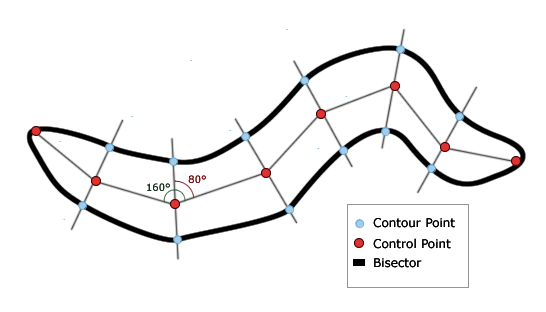
\includegraphics[scale=0.7]{descriptor/descriptor}
 \caption{Construction of a worm shape based on shape descriptor}
 \label{fig:descriptor}
\end{figure}

In order to obtain a contour that accurately represents the worm shape along the 
medial axis, the choice of the opposite points in the \emph{thickness} circles 
must take into account the \emph{skeleton} bendings.
Since the shape is constructed following the \emph{thickness} of control points,
the bendings in the generated shape occur at each of these ones, and can then be 
calculated as the angle between the straight lines that connect the control points.
The bisection of any angle provides a straight line that divides it
into two equal portions, measuring the bending variation at each control point.
Then selecting the two points at a respective \emph{thickness} distance, from every control
point, following the bisection line in opposite directions provides a set of points
that joined together with a smooth curve will give a worm shape contour.\\

Generating a smooth curve around the control points improves the accuracy of the shape
description, compared to tracing straight lines
between the contour points. At the same time it allows to obtain a good representation
of the shape with a considerably smaller number of control points. The smooth curve
is obtained by calculating the cardinal spline (covered in Sec. \ref{splines}) given the
contour points. A cardinal spline is a function that describes a smooth curve that
passes over all the points of a set, given a starting and ending point. In this case
the starting and ending points are the same, so the described contour is closed.\\

The worm profile for a set of control points can be both manually set or automatically
calculated from the \emph{isolated worms} as explained in the section below.

\subsubsection{Automatic Profile generation}
\label{sec:metwormprof}

The shape of \emph{isolated worms} identified in the image can be accurately matched
by following the contour points in their respective distance map, as explained 
in Sec. \ref{sec:metiso}. Given a set of matched shapes for \emph{isolated worms}, and
the initially detected skeleton, a worm profile (as described previously) can be 
generated by measuring the \emph{thickness} of every control point and finding the mean
among these.\\

In order to measure the thickness for every control point, a set of
$N$ equidistant points is generated that cover the skeleton of the \emph{isolated worm}.
Then as described in the previous section, the bisectors of the angles between the 
straight lines connecting the control points are calculated. Starting from every control
point, the bisector line is ``walked'' until the pixel with the lowest distance map
value is found, a contour point in most of the cases. The operation is repeated for every 
control point bisector in both opposite directions. The Euclidean distance from a control
point to each found pixel is calculated, and its average is recorded. Repeating this process
with every  \emph{isolated worms} generates a set of \emph{thickness profiles}, one for each
\emph{isolated worms}. Then a general worm profile is calculated by finding the mean between
the thickness values for every control point in each \emph{thickness profile}. In order 
to generate an accurate profile, that avoids oversized (or downsized) worms and wrongly
detected \emph{isolated worms}, the $20\%$ higher and lower values are discarded when 
calculating the average. The \emph{thickness} value for
the endpoints, \emph{i.e.} the first and last point in the set of length $N$, is zero,
so one contour point is generated in the extremes instead of two.
Having done this a \emph{thickness profile} is obtained that represents the average 
radius distance for every control point to its closest contour pixel, allowing 
to generate a generic worm shape around any skeleton defined by $N$ points. 

\subsection{Triangle mesh and rasterization}
\label{sec:metrast}


\subsection{Profile-driven shape fitting}
\label{sec:metfit}

Once the initial processing of segmentation and worm skeletonization is performed, where 
information about the worms in the image is gathered, a shape matching process has to be 
carried out in order to detect the shape that corresponds to each worm, 
following the prior information. The matching process is different for
\emph{isolated worms} and \emph{worm clusters}  
due to their nature. In this sections both processes are explained and some 
implementations details are given.


\subsubsection{Isolated Worms shape fitting}
\label{sec:metiso}

At this point the information gathered about each \emph{isolated worm} consists in 
a 1-pixel skeleton path between exactly two endpoints. Since this process is carried
out after each endpoint is identified correctly, the area conformed by the object pixels
surrounding the skeleton will correspond to the exact shape of the \emph{isolated worm}.\\

In order to optimize the calculation of the worm area, the contour of the shape is first
traced and then the internal area is triangulated and rasterized following the process
explained in \ref{sec:metfit}. The contour is traced by finding the closest border-pixel
to any endpoint and then following the neighbor that is also a border-pixel. A
border-pixel is such that has a value of one (1) in the image distance map.
This allows to obtain the contour and area of the worm shape corresponding to each 
\emph{isolated worm} accurately.


\subsubsection{Worm Cluster shape fitting}
\label{sec:clusterfit}

The \emph{worm clusters} represent a more complicated shape matching scenario due to their
variable number of worms and the many different possible conformations that can be obtained. 
The  overlaps in \emph{worm clusters} makes difficult to differentiate the group of pixels
that belong to the area of one worm or another. A matching process must then be 
carried out that calculates the most likely worm conformation that starts from every
endpoint in order to obtain the set of conformations that best fit the whole 
\emph{worm cluster}.\\

An shape optimization matching approach was followed that consists of calculating all the 
worm conformations starting from any endpoint. A worm conformation is obtained by generating
a generic worm shape from a skeleton path and deforming that shape until the dissimilarity
between the generated shape and the binary image is minimum. Below, the main steps and 
features of the algorithm are described:

\begin{itemize}
\item For every endpoint the set of feasible skeleton paths starting from that pixel
  are calculated.
\item Given a skeleton path, a generic worm shape is constructed by generating a shape
descriptor following the worm profile of the image.
\item An optimization process deforms the generic worm shape until the dissimilarity
between the shape and the corresponding binary image is minimized. The optimized
shape corresponds to a feasible worm conformation.
\item Once all the possible conformations from every endpoint are calculated, a set of
conformations is selected that maximizes the number of endpoints covered and minimizes
the sum of the energy values. The selected conformations are the best automatic matches.
\end{itemize}

\subsubsection*{Shape deformation}

The calculated skeleton paths starting from a given endpoint are guesses of possible
worm skeletons. Since the deformed model is constructed over a skeleton path 
(that is close to the medial axis of the \emph{worm cluster}) the initally generated 
shape will always be close to a worm shape. Given this, just slight perturbations of
the generated shape would deform the model sufficiently to correct the deviation of the
skeleton from the actual medial axis, obtaining thus the most likely worm shape
over the given path.\\

The deformations are made over a shape descriptor, that is defined by a series of 
control points and constructed following a worm profile. In order to provide feasible
shapes and to limit the number of possible deformations, a deformation will consist
in the repositioning of a given control point. The number of different positions that a 
given control point can take is fixed and set along the bisection of the angle between
the lines that connect the previous, current and next control point. 
Following this, the set of deformations that can be performed from an initial shape 
can be calculated fastly and provides a great number of possible different conformations.\\

\subsubsection*{Energy Formulation}
 
The distance function must provide a measure of how far is the deforming shape from a worm in the image, 
\emph{i.e.} how well
the deforming shape fits. To measure the dissimilarity between a given worm shape and the
matching image, an energy formulation was followed, based on Active Contour Models,
\cite{snakes}, that consists of an external energy and an internal energy.\\

The external energy models how well the deformed model matches the data. Since the more
background pixels are covered the farther the model is from a worm in the \emph{worm cluster}, 
then a good measure for the external energy would be the percentage of background pixels in the 
area covered by the deformed model.Then, the more object pixels are covered the lower the 
external energy is. So, given a model $M$ and the functions $bg$ and $fg$  that measure
the amount of background and foreground pixels respectively, the external energy
can be defined as:

$$E_{ext}(M) = \frac{bg(M)}{bg(M)+fg(M)}$$

The measure is not considered just as the sum of background pixels
because the energy value will be too variable, given the variability of the amount
of pixels covered by a worm shape.\\

The internal energy is the one that models the objects resistance to be deformed into
a shape that do not corresponds to the modeling class, \emph{e.g.} the worm class. 
This means that the internal energy resists to obtain not feasible worm
shapes after deformation. The internal energy for
snakes, as explained in \cite{snakes}, works as a smoothness constraint and is explicitely
formulated (usually in terms of first and second derivatives). As stated in \cite{bspline}, 
many problems arising from this formulation have been recognized in literature such as:
slow convergence speed, difficulty in determining the weights associated with the 
smoothness constraint, high order derivatives on discrete curves may not be accurate
in noisy environments.\\
However, in the approach proposed in this work, every shape is generated from a worm 
profile following a shape descriptor,so every deformed shape will still belong to the 
worm class. Thus is not necessary to include the internal energy in the 
formulation.

\subsubsection*{Matching Optimization}

The optimization process consists in obtaining the most likely worm shape that can be
obtained by deforming a shape constructed over a skeleton path, knowned as a 
worm conformation. Given how quickly the different deformations can be computed,
a local-search optimization approach is followed. The process consists in obtaining the
best individual in the neighborhood that improves the energy function, until is 
minimized. The neighborhood is calculated in the following way:
For a given shape, four (4) different deformations are calculated for control point.
The possible deformations or new positions are the
next and second next position in north and south direction, \emph{i.e. }the two opposites
directions of the bisection of the control point.
There are then $N*4$ different possible deformations (neighbors) for a given shape,
where $N$ is the number of control points.\\ 
Then a neighborhood consists of mild and slightly stronger deformations of a given
worm shape for any control point.\\ Since the focus is to obtain the most accurate worm 
shape for a given skeleton, the
first and last control points, that correspond to the worm endpoints, are fixed.\\

Once the best shape is obtained a contour fixing process is carried out, that
consists in the expansion or contraction of the contours of the shape in order to adapt
to the actual worm in the image. This is required since the optimized shape is built 
following a worm profile, that just represents the shape of the worms in the image 
generically. In this process the extremes constructed from the control points are pushed
to contour points following the distance map, either expanding or contracting. While
expanding or contracting, every considered new possible position must have either the 
same or lower distance map value. A better point must be found after a fixed number
of steps, otherwise is discarded. This is done to avoid too big and strange deformations.


\subsection{Manual Fixing}

A process of manual fixing can be performed by the user to improve the shape fitting
accuracy, such as adding missing endpoints or fixing wrong worm conformations. Below
both mentioned manual processes are explained. 

\subsubsection{Endpoint operations}
\label{sec:endpointop}

Worm endpoints are detected by first identifying extremes in the worm
skeleton. However when the extreme of a given worm in an image overlaps with 
another worm shape, the shapes become continous so the shape skeleton will be generated 
as a continuous path, thus the extreme point will be missing and the endpoint will not be 
detected. Since the solution methodology is centered on finding paths between endpoints and 
then determining the most likely worm paths, having missing endpoints could affect 
the matching accuracy.\\

Worm endpoints are simple to detect for a human being, once had the skeleton of the 
a worm cluster, so the missing endpoints could be added rapidily by following a manual
process. This process consists in looking at the extreme of worms and adding a 
extreme point when missing. Since by definition an endpoint is the extreme of a worm path,
it must have one and only one neighbor belonging to the skeleton. When an added extreme
point has more than one skeleton neighbor the user would have to select the extra
neighbor pixel for deleiton.
In summary the user can add the missing endpoints by selecting the missing pixel
and perhaps selecting some neighbors as well if is necessary to disconnect. 

\subsubsection{Matching fixing}
\label{sec:matchfix}


%%avoid page number on blank pages when cleared
\thispagestyle{empty}
\cleardoublepage
\chapter{Experiments and Results}
\label{chap:experiments}

%Introduce Chapter: 3 experiments (test set size = 3) to test the whole
%shape matching methodology. Its separated in three main processes: initial
%processing, automatic shape matching and manual fixing. The results are 
%presented and discussed.

In this chapter, the different experiments carried out to test the performance
of the shape matching solution are 
presented, explaining the reason for their choice and the test objectives.
Then, the results are presented and discussed, pointing out the advantages and drawbacks of the suggested
shape matching model that are inferred from the first ones.

\section{Experiments}
\label{sec:experiments}

In order to test the implemented solution, three digital images of worms in liquid
media were provided by Johan Henriksson at the \emph{Department of Bioscience and Nutrition, Karolinska Institutet}.
Each image corresponds to a different difficulty level, 
following the criteria of number of worms and degree of overlap. Thus, the greater the number 
of worms in the image and the greater the number of worms that are connected by overlapping,
the greater the difficulty level. The overlapping degree is determined by the number
of worms that belong to the different \emph{worm clusters} (first defined in Sec. \ref{sec:reasoning})
and the number of \emph{worm clusters} in the image.
The selected images are named \emph{test image 1}, \emph{test image 2} and \emph{test image 3}
and are displayed in an increasing difficulty level order, from the easiest to the hardest. 
The characteristics of the test set are presented in Table \ref{tab:testset}.


\begin{table}[h]
  \caption{Characteristics of the test set images}
\begin{center}
\begin{tabular}[h]{|>{\columncolor[gray]{0.9}} p{2cm} |p{3cm} | p{2.8cm} | p{3cm}| p{2.8cm} |}
    \hline
    \rowcolor[gray]{.9}
    Test Image & Number of Isolated Worms & Number of Worm Clusters & Number of Worms in Clusters  & Total Number of Worms\\
    \hline
    Test 1 & 11/19 (57.8\%) & 3 & 8/19 (42.1\%) & 19 \\
    \hline
    Test 2 & 8/33 (24.2\%) & 3 & 25/33 (75.7\%)& 33 \\    
    \hline
    Test 3 & 13/38 (34.2\%)& 5 & 25/38 (65.7\%) & 38 \\
    \hline 
  \end{tabular}
\end{center}
  \label{tab:testset}
\end{table}


For each test image a series of experiments were carried out to test the performance of
the different processes that are involved in the solution methodology. The entire 
shape fitting process was divided into three stages that represent the 
main fitting steps. These are: \emph{initial Processing}, \emph{automatic shape matching} and
\emph{manual adjustment}.\\

The \emph{initial processing} involves all the image processing steps that are performed 
before the shape matching optimization process, as explained in Sec. \ref{sec:solmet},
such as: thresholding, distance transformation, skeletonization, 
clustering, endpoint detection and worm profiling. Among these, the distance transformation
and skeletonization follow already implemented and tested algorithms (covered in Sec. \ref{sec:metdt}
and Sec. \ref{sec:metsk}) and produce straight-forward results, so there is no need to analyze them further.
The clustering process follows the skeletonization process and is straight-forward as well.
On the other hand the thresholding, endpoint detection and worm profiling processes vary 
from image to image, so different experiments are carried out in order to test these sub processes
for the test set.\\

The \emph{automatic shape matching} stage consists of experiments dealing with the automatic
optimization process to match \emph{worm clusters} and contour-following technique to match 
\emph{isolated worms} that produce the initial fitting of the worms. These 
experiments attempt to measure the efficacy and time efficiency of different variations of the
matching algorithm, in order to make a conclusion about properties of the algorithm and the feasibility 
of the automatic solution.\\
The third stage, \emph{manual adjustment}, attempts to measure the type and number of 
manual adjustments that must be performed by the user in order to correct the 
wrongly assigned matches. The experiment is also 
aimed at determining how much the efficacy of the automatic solution can be improved, in
order to get a better matching. Once the best possible matching is found through manual adjustment,
the stability of the best match is studied by comparing the energy to the second and third best
matches.\\

The experiments were executed on a personal computer with a 2.00 GHz AMD Turion 
Dual-Core Mobile Processor, 1 MB Microprocessor cache and 3Gb of RAM Memory, 
on Linux Operating System, Ubuntu Distribution.

\section{Results}
\label{sec:results}

In this section the results obtained for the test set are presented and discussed.
The results are distributed in the three main stages: \emph{initial processing}, \emph{automatic shape matching} and
\emph{manual adjustment}. In the section \emph{initial Processing}, the results for the three different 
images in the test set are presented. On the other hand the section \emph{shape fitting} presents the different
results for the stages \emph{automatic shape matching} and \emph{manual adjustment} for every test image
individually.

\subsection{Initial Processing}
\label{sec:initproc}

This section presents the results for the experiments carried out over the test set for the 
processes: thresholding and endpoint finding. Then a brief discussion about
the result for the worm profiling process is presented.

\subsubsection*{Thresholding}

As explained in Sec. \ref{sec:thresimp}, \emph{Endrov} has implementations for the 
thresholding filters \emph{Fukunaga}, \emph{max entropy}, \emph{Otsu} and \emph{percentile}.
In order to select an appropriate thresholding
filter, the four previously mentioned were tried on every test image, tweaking the
input parameters until the best possible binary image was obtained for every one.
From visual inspection, the \emph{percentile} filter generated the
best binary images for the three tests. 
The best percentile values for every test image are shown in Table \ref{tab:threshold}.
The second closest method was \emph{Fukunaga}
that produced acceptable solutions after the combination of binary images
generated from different number of classes, however the results were not as good as
the ones obtained with \emph{percentile} and also required more processing.

\begin{table}[h]
  \caption{Best percentile values for percentile thresholding of test images}
\begin{center}
\begin{tabular}[h]{|>{\columncolor[gray]{0.9}} c |c|c|c|}
    \rowcolor[gray]{.9}
    \hline
    Test & Test Image 1 & Test Image 2 & Test Image 3\\
    \hline
    Percentile Value & 0.074 & 0.1 & 0.11\\
    \hline
  \end{tabular}
\end{center}
  \label{tab:threshold}
\end{table}

The resultant best percentile values oscillate between $0.074$ and $0.11$, and are 
simple to determine using \emph{Endrov}.   

\subsubsection*{Endpoint detection}

This section presents the results for the detection of worm endpoints.
Table \ref{table:endtable} shows the number of worm endpoints that are
automatically detected and those that have to be manually added, in order
to cover all the endpoints for the worms in the image.

\begin{table}[h]
  \caption{Worm endpoints detection and fixing for the test set}
\begin{center}
\begin{tabular}[h]{|>{\columncolor[gray]{0.9}} p{2cm} |p{1.9cm}|p{2cm}|p{2.2cm}|}
    \rowcolor[gray]{.9}
    \hline
    Test Image & Total Endpoints & Detected Endpoints & Manually Added Endpoints\\
    \hline
    Image 1 & 38 & 38 (100\%) & 0 \\
    \hline 
    Image 2 & 66 & 53 (80\%) & 13 \\
    \hline 
    Image 3 & 76 & 57 (75\%) & 19 \\
    \hline
  \end{tabular}
\end{center}
  \label{table:endtable}
\end{table}

Table \ref{table:endtable} presents the number of endpoints identified
automatically for every test image and the number of endpoints that must be added manually.
It shows that a large number of worms belonging
to \emph{worm clusters} increases the probability to have endpoints overlapping, 
as does a high density of worms.
Considering the large number of worms that belong to worm clusters 
for images two and three (as show in  Table \ref{tab:testset}) and the low
number of clusters for each one (which increases the overlapping), the amount
of missing endpoints can be considered fairly low and it is feasible to add them manually.

\subsubsection*{Worm Profiling}

In order to generate an accurate worm profile of the worms present in the image
it is necessary to have \emph{isolated worms} in the processed image. The percentage 
of \emph{isolated worms} for every image were $57.8\%$, $24.2\%$ and $34.2\%$ 
respectively,
oscillating between $8$ and $13$ worms, as shown in Table \ref{tab:testset}. 
For all images, the generated worm profiles were sufficiently accurate to
conduct the optimization shape matching process, whose results are presented in 
the subsections named \emph{automatic shape matching} for every test image result.

\subsection{Shape Matching}

In this section, the results for the second and third stage in the 
solution methodology are presented, as described above in Sec. \ref{sec:experiments}, which consist
in \emph{automatic shape matching} and \emph{manual adjustment}. 
For the \emph{automatic shape matching} subsection the results for a series of four 
variations of the matching algorithm are presented, focusing on the matching accuracy 
and time performance. The two main variants are: \emph{path guessing} and 
\emph{every path}. 
\emph{Path guessing} is the version of the algorithm in which every guessed path is favored
by an improvement in its shape optimization value, by reducing it to the half. So when 
a conformation is to be chosen for an endpoint the value of the guessed path is more likely
to be selected. On the other hand, the \emph{every path} variant considers every possible conformation for every endpoint.
Each variant is executed with and without manually adding the missing endpoints.\\

The \emph{manual adjustment} presents the results of modifying the erroneous matches
obtained by the best automatic matching algorithm, showing the resulting best
possible matching image and indicating the number of worm shapes that had to be 
re-arranged. This process is done manually: The user detects the wrong match visually 
and selects two endpoints to obtain the best optimized shape that connects them, as
explained in Sec. \ref{sec:matchfix}. An operation (as used in the tables for this section) 
is considered to be the process of selecting two endpoints and generate a new shape.\\

Then a subsection \emph{matching energy} is presented, in which the distribution of
the energy values for the different conformations is discussed. This section presents
a graph showing the different energy values (objective function) for the correct conformation
and the next two best conformations for every endpoint (of those having three or more conformations). 
The correct conformation corresponds to the one that is constructed between the two endpoints that
belong to the worm in the image. The other two are conformations that start in the
selected endpoint and end in a wrong one.


\subsubsection*{Automatic Shape Matching (Test Image 1)}

Since for the test image 1 all the endpoints are found automatically, as shown in 
Table \ref{table:auto1}, the results presented here show the matching efficiency and
runtime just for the variations \emph{every path} and \emph{path guessing}, which include all the
worm endpoints. Table \ref{table:auto1} presents the obtained results.

\begin{table}[h!]
  \caption{Results of automatic worm shape matching on test image 1}
  \begin{center}
  \begin{tabular}{|>{\columncolor[gray]{0.9}} p{3cm}|p{2.8cm}|p{2.8cm}|p{2.8cm}|c|}
    \hline
    \rowcolor[gray]{.9}
    Path Finding & Isolated Worms Matching & Cluster Worms Matching 
    & Total Matching 
    & Time (s) \\ 
    \hline
    Every Path & 11/11 (100\%) & 6/8 (75\%) & 17/19 (89.5\%)& 6.47 \\
    \hline
    P. Guessing & 11/11 (100\%) & 8/8 (100\%) & 19/19 (100\%) & 7.53 \\
    \hline
  \end{tabular}
\end{center}
  \label{table:auto1}
\end{table}

It can be observed that in both variations of the algorithm the 
\emph{isolated worms} were all matched. For the \emph{every path} variation 
three quarters of the worms in clusters were matched correctly.
On the other hand, the \emph{path guessing} variation managed to match automatically 
all the worms in the image. The execution time is slightly higher for the
\emph{path guessing} Variation, as expected because of the extra calculations that
must be performed to calculate the best paths departing from each endpoint.\\

For this image, the \emph{path guessing} variant represented an improvement in 
the solution, by inducing the shape produced from guessed paths to be more
likely to be selected. On the other hand, at first glance, the isolated
worms seem to be matched regardless of the algorithm variant, as expected.\\
The best matching for test image 1, corresponding to the \emph{path guessing} variation, is shown in Fig. \ref{fig:best1}.


\begin{figure}[h!]
  \centering
  \subfloat[Best match]{\label{best1}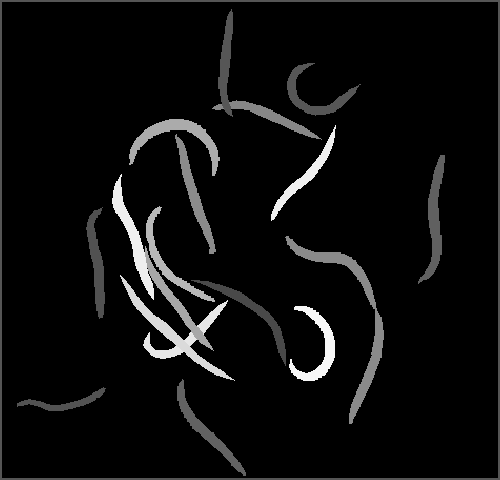
\includegraphics[scale=0.34]{results/test1/complete-frame1}}
\qquad
  \subfloat[Best match over original image]{\label{bestbg1}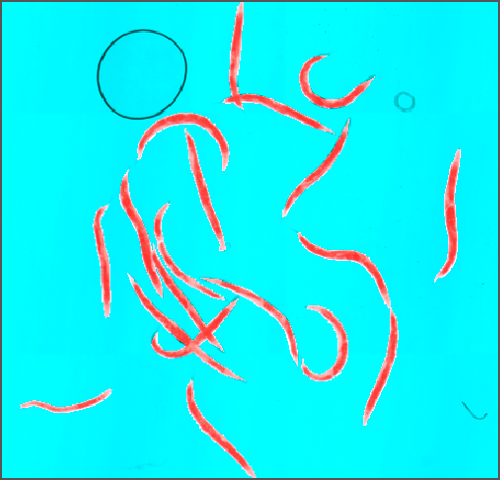
\includegraphics[scale=0.34]{results/test1/complete-framebg1}}
  \caption{Best automatic shape matching on test image 1}
  \label{fig:best1}
\end{figure}


\subsubsection*{Automatic Shape Matching (Test Image 2)}

The results for automatic matching on test image 2 are shown in table \ref{tab:tab2}.

\begin{table}[h]\begin{tabular}{|>{\columncolor[gray]{0.9}} p{3cm}|p{2.8cm}|p{2.8cm}|p{2.8cm}|c|}
    \hline
    \rowcolor[gray]{.9}
    Path Finding & Isolated Worms Matching & Cluster Worms Matching 
    & Total Matching 
    & Time (s) \\ 
    \hline  
    Every Path - me & 8/8 (100\%) & 7/25 (28\%) & 15/33 (45.4\%) & 21.8 \\ 
    \hline
    P. Guessing - me & 8/8 (100\%) & 10/25 (40\%) & 18/33 (54.5\%) & 23.7\\
    \hline
    Every Path + me & 8/8 (100\%)& 15/23 (65.2\%) & 23/33 (69.7\%)& 42.3 \\
    \hline
    P. Guessing + me & 8/8 (100\%)& 21/25 (84\%) & 29/33 (87.8\%) & 45 \\
    \hline
  \end{tabular}
  \label{tab:tab2}
  \caption[Results of automatic worm shape matching on test image 2, with and without missing endpoints]{Results of automatic worm shape matching on test image 2, with and without missing endpoints (me)}
\end{table}

It can be observed that for every variation the \emph{isolated worms} were matched
totally. For the two variations that have missing endpoints, just around
the half of the total worms could be matched. Although the execution time is
slower, which is expected given the decrease of feasible paths, not having an
endpoint of a worm makes impossible to find a shape that matches it correctly.
For the variations that include endpoints the results are considerably better.
It can be observed that the \emph{path guessing} variation
increases the matching accuracy, in both missing and not missing
endpoints set of variations. The execution time also increases
when all endpoints are added, as expected. 
For the \emph{path guessing} variation the matching percentage increases considerably,
although is slightly slower than \emph{every path}.
In the best case the automatic matching solution manages to fit the shape
for all the isolated worms and a high percentage of the clustered worms in
less than a minute.

\subsubsection*{Manual Adjustment (Test Image 2)}

\emph{Path guessing} with no missing endpoints gave the best result,
with just $4$ worms wrongly matched among $33$. Fig. \ref{fig:best2} shows the matches.

\begin{figure}[h]
  \centering
  \subfloat[Best automatic match]{\label{test2:best2}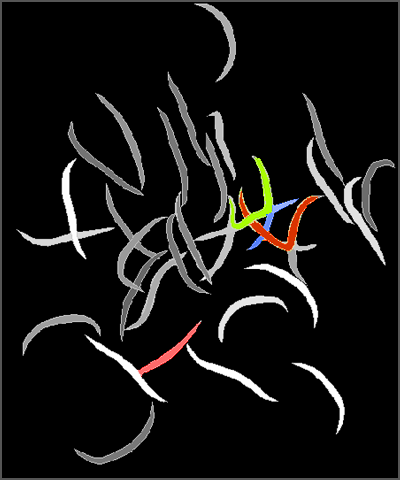
\includegraphics[scale=0.45]{results/test2/guessing-nobgframe}}
\qquad
  \subfloat[Best automatic match over original image]{\label{bestbg1}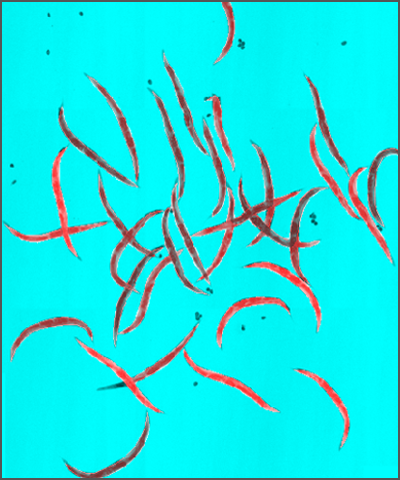
\includegraphics[scale=0.45]{results/test2/guessing-bgframe}}
\qquad
  \subfloat[Manually adjusted match]{\label{test2:bestbg2}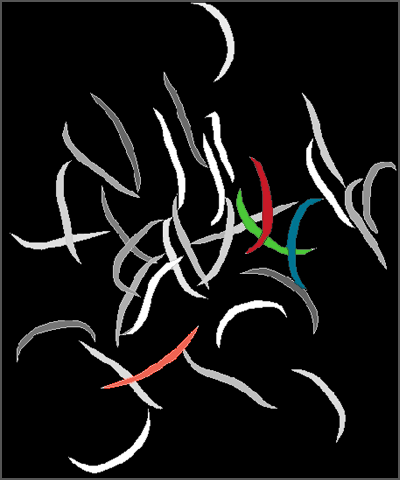
\includegraphics[scale=0.45]{results/test2/frame2-allnobg}}
\qquad
  \subfloat[Manually adjusted match over original image]{\label{bestbg1}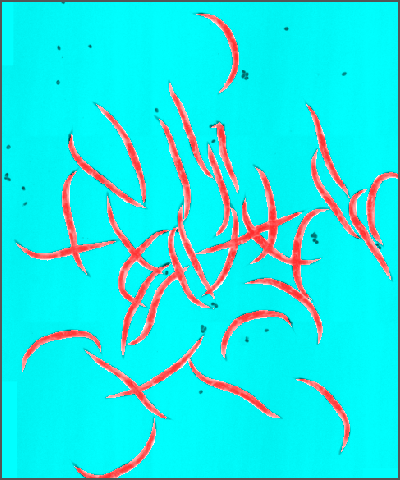
\includegraphics[scale=0.45]{results/test2/frame2-all}}

\caption[Best automatic shape matching and manual match fixing on test image 2]{Best automatic shape matching and manual match fixing on test image 2. Colored shapes and outlines in images
    \ref{test2:best2} and \ref{test2:bestbg2} indicate incorrectly detected worms}
\label{fig:best2}
\end{figure}

Manual adjustment required selecting two endpoints that correspond to an actual worm shape. After selecting the
endpoints the assigned shapes starting at this endpoints are removed
and the best shape that connects the two selected endpoints is added.
Finally all of the worms in the image could be fitted.


\subsubsection*{Automatic Shape Matching (Test Image 3)}

The results for automatic matching on test image
3 are presented in table \ref{tab:tab3}. The four variations for the algorithm are shown.

\begin{table}[h!]\begin{tabular}{|>{\columncolor[gray]{0.9}} p{3cm}|p{2.8cm}|p{2.8cm}|p{2.8cm}|c|}
    \hline
    \rowcolor[gray]{.9}
    Path Finding & Isolated Worms Matching & Cluster Worms Matching 
    & Total Matching 
    & Time (s) \\ 
    \hline  
    Every Path - me & 13/13 (100\%) & 5/25 (20\%) & 18/38 (47.3\%) & 26.4 \\ 
    \hline
    P. Guessing - me & 13/13 (100\%) & 7/25 (28\%) & 20/38 (52.6\%) & 28.7\\
    \hline
    Every Path + me & 13/13 (100\%)& 13/25 (52\%) & 26/38 (68.4\%)& 36.2 \\
    \hline
    P. Guessing + me & 13/13 (100\%)& 16/25 (64\%) & 29/38 (76.3\%) & 39.8 \\
    \hline
  \end{tabular}
  \label{tab:tab3}
  \caption[Results of automatic worm shape matching on test image 3, with and without missing endpoints]{Results of automatic worm shape matching on test image 3, with and without missing endpoints (me)}
\end{table}

The isolated worms were always matched successfully.
\emph{every path} and \emph{path guessing} with missing points, 
the total matching is around the half of the total. 
With missing endpoints adjusted, the level of accuracy increases considerably.
Calculation is slower with more endpoints.
The \emph{path guessing} variations is always better than \emph{every path}, and is slightly slower.\\
The best variation was the \emph{path guessing} with no missing endpoints, managing
to match all the \emph{isolated worms} and a total of three quarters of the 
whole image.

\subsubsection*{Manual Adjustment (Test Image 3)}

The \emph{path guessing} without missing endpoints turned out to be the best one, with $9$ worms wrongly matched among $38$.
Fig. \ref{fig:best3} presents four images for this algorithm.
\begin{figure}[h!]
  \centering
  \subfloat[Best automatic match]{\label{test3:best3}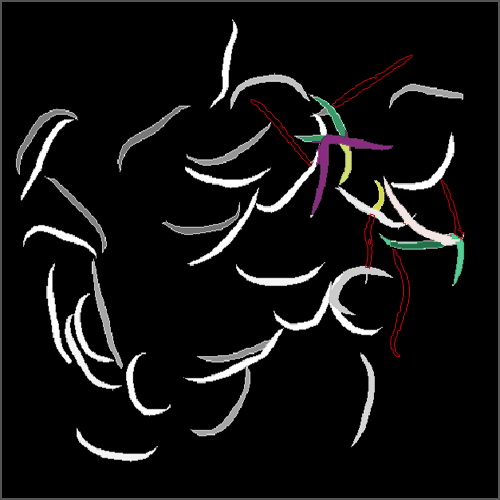
\includegraphics[scale=0.35]{results/test3/guess-nobg}}
\qquad
  \subfloat[Best automatic match over original image]{\label{bestbg1}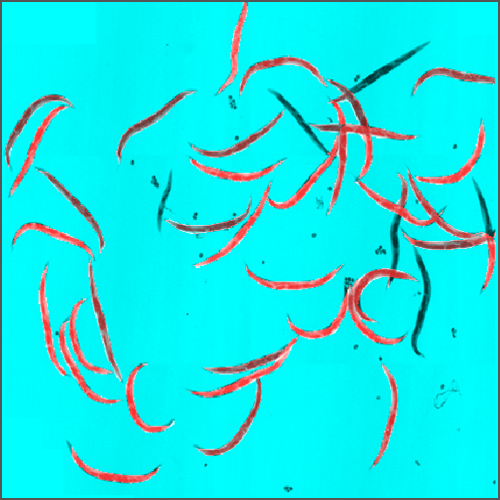
\includegraphics[scale=0.35]{results/test3/guess-bg}}
\qquad
  \subfloat[Manually adjusted match]{\label{test3:bestbg3}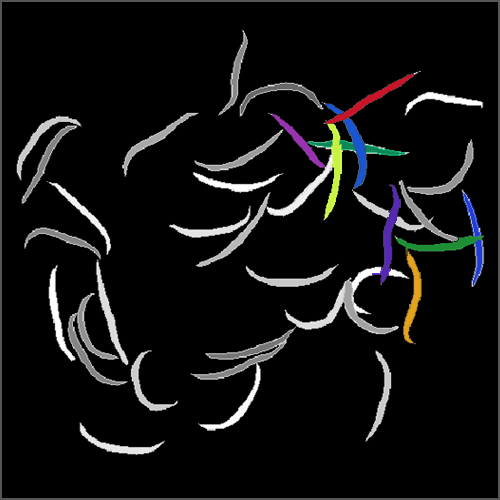
\includegraphics[scale=0.35]{results/test3/all-nobg}}
  \label{best3:c}
\qquad
  \subfloat[Manually adjusted match over original image]{\label{bestbg1}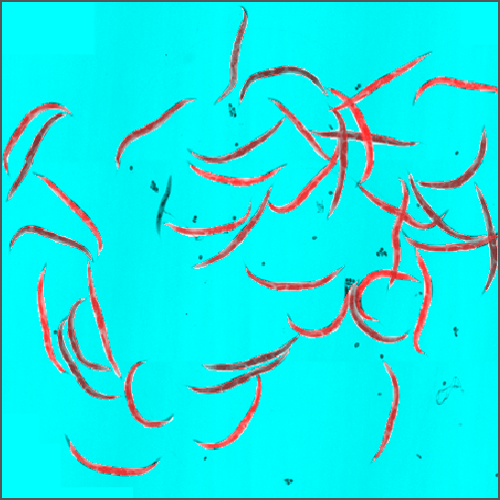
\includegraphics[scale=0.35]{results/test3/all-bg}}
  \caption[Best automatic shape matching and manual match fixing on test image 3]{Best automatic shape matching and manual match fixing on test image 3. Colored shapes and outlines in images
    \ref{test3:best3} and \ref{test3:bestbg3} indicate incorrectly detected worms}
  \label{fig:best3}
\end{figure}


Nine operations were required to manually adjust the incorrectly matched worms.
All the worms in the image could then be matched and fitted.

\subsection{Matching Energy}

The energy for the best three conformations in each endpoint is shown in Fig. \ref{fig:energy123}.
The first is correct and matches the worm, the other two match wrong endpoints.\\
Recall that the energy function, covered
in Sec.\ref{sec:clusterfit}, evaluates the distance between a matching shape
and a matched shape as the percentage of background pixels contained in the 
area covered by the matching shape, so all the possible energy values are
contained in the interval $[0,1]$ and the optimized shapes tend to take values
from one to three decimals close to $0$.

\captionsetup[subfloat]{farskip=-0.8cm,captionskip=-0.2cm}

%Distance between images could be reduced to make graphs larger
\begin{figure}[htp]
  \begin{center}
    \subfloat[Image 1]{\label{fig:energy1b}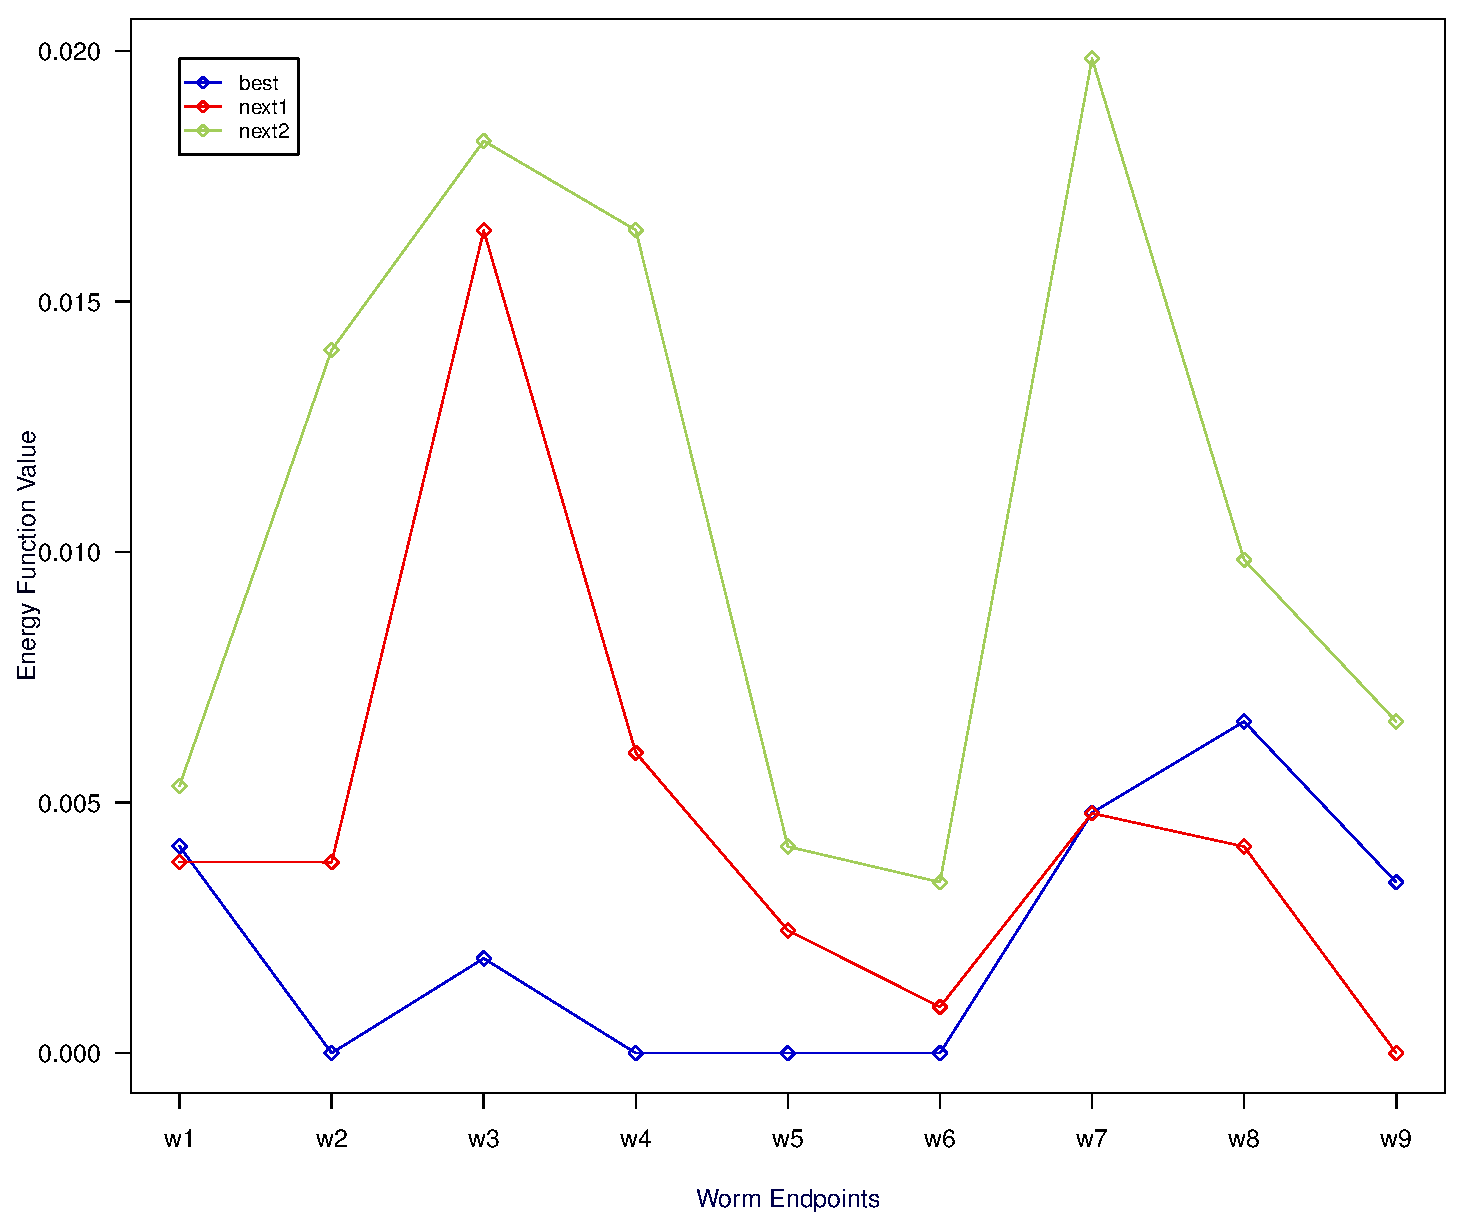
\includegraphics[scale=0.54]{results/test1/energy-graph}}\\
    \subfloat[Image 2]{\label{fig:energy2b}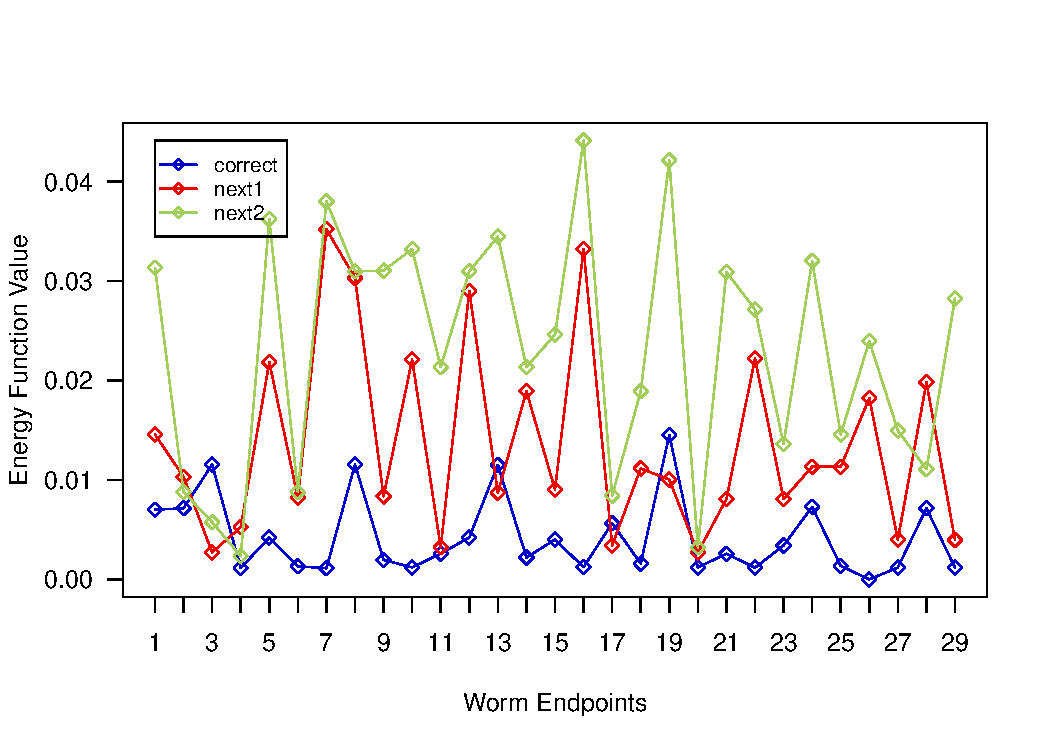
\includegraphics[scale=0.54]{results/test2/energy-graph}}\\
    \subfloat[Image 3]{\label{fig:energy3b}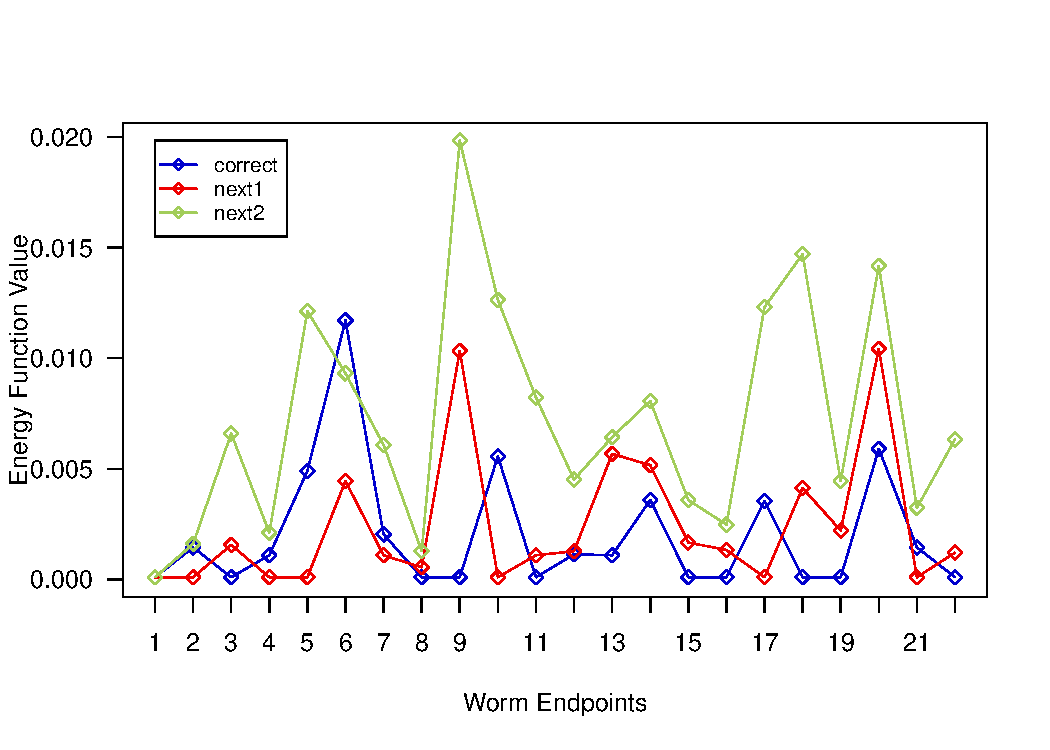
\includegraphics[scale=0.54]{results/test3/energy-graph}}
  \end{center}
  \caption[Energy value for the best three conformations by endpoint ID on test
images]{Energy value for the best three conformations by endpoint ID on test
images. The correct conformation is red. The selected endpoints correspond to worms in worm clusters that
have more than two possible conformations.}
  \label{fig:energy123}
\end{figure}
\showcaptionsetup{subfloat}

\subsubsection*{Test Image 1}

For most endpoints the correct conformation has the lowest energy value.
In two cases a wrong conformation had a lower energy value than the correct
one. The third best conformation always has higher energy than the correct conformation.\\

\subsubsection*{Test Image 2}


It can be observed that the second best conformation (in green) is in all 
the cases worst that the best conformation, normally from two to four times 
in terms of the energy function value, thus the correct conformation is 
either the best or the second best conformation, from all the possible.
In this case only four endpoints among twenty nine show a better energy
function value for the best next conformation (in red) over the correct 
conformation (in blue). This coincides directly with the results shown
in Table \ref{tab:tab3} where, for the best automatic solution (\emph{path guessing}),
the amount of worms successfully matched was 29/33, which is only four worms
away from the optimal solution, the same number of endpoints in which the
correct conformation is not the best in value. In fact, the difference of 
values between the correct and best next conformation for the these four
endpoints is close enough to think that a more sensitive objective function
could retrieve the correct conformation for all the cases for the automatic
algorithm.\\ 

\subsubsection*{Test Image 3}

Among the 22 endpoints, for 9
of them the second best conformation resulted to have a better energy value
than the correct conformation. This is consistent with the results presented
in Table \ref{tab:tab3} where for the best variation (\emph{path guessing}), the
number of wrongly detected worms is also nine. This means that an incorrect 
path is considered to be more likely to be a worm starting from this
endpoints. For every endpoint, with the exception of one, the second best 
solution is worse than the correct solution. So the energy value of the 
correct solution is either the best or the second best.\\

Given that for this image the amount of worms that belong to clusters
is high (25), the number of possible paths starting
from every endpoint is also high and so is the number of wrong conformations.
Since so many correct conformations did not have the lowest energy value,
the energy formulation must not be sensitive enough. However
the differences between the correct and selected conformations for
these cases are close (just as for test image 2), so a more sophisticated objective function could lead
to better results.\\

%%avoid page number on blank pages when cleared
\thispagestyle{empty}
\cleardoublepage
\chapter{Conclusions and Future Work}

In this chapter, the conclusions obtained from the experiment results of the 
worm shape fitting methodology developed in this work are addressed.
Then some future work suggestions are presented, pointing out the modifications
that can be performed to improve the solution methodology.

\section{Conclusions}

\subsection*{Solution Methodology}

The proposed methodology provides a feasible semi-automatic solution
to identify and fit worm shapes in bright-field digital images. This allows
to turn the microscope worm images into manageable computer data and 
improve considerably the time cost and matching accuracy with respect
to manual identification.\\
The methodology design and implementation are efficient enough to provide
a complete identification of worms in short time using a personal computer.\\
The solution is said to be semi-automatic because of the need of manual
tweaking in two steps of the process: endpoint identification and
final matching. Once the endpoints are completely identified, the automatic
solution provides a high matching percentage (more than three quarters of 
the total, in the worst case), that can be even be optimal in \emph{easy} 
images. The final matching process allows the user to re-arrange the 
automatic solution, providing an optimal match for the image.\\
The \emph{Initial Processing} step is quickly executed, less than
$1\%$ of the total execution time. On the other hand The \emph{Shape Matching}
step is the most time consuming process, consuming the $99\%$ of the total
time excluding the time taken for manual adjustments (normally fast).

\subsection*{Isolated Worms and Worm Cluster matching}

The \emph{isolated worms} are fully identified in every image following
an automatic process, without requiring manual addition of endpoints
or match fixing. An accurate image worm profile can be successfully 
calculated from the \emph{isolated worms}.\\
The identification of worms in \emph{worm clusters} represented the most 
challenging process of the worm fitting methodology. A high density
of worms leads to multiple overlaps and clustering, where endpoints can fail
to be detected. Worms will not be identified correctly if endpoints are
missing, so manual adjustments are required.\\
The shape of \emph{isolated worms} can be traced accurately in all the cases.
For worms in clusters the shape is initially matched through the perturbation
of a descriptor that is built from a worm profile. Once the optimal shape
is found the contours of the generated shape are expanded or contracted
to fit the individual shapes. This process is performed successfully, and in
all the cases the best shape between endpoints is either exact or very close
to the worm shape in the image.

\subsection*{Path Guessing}

The path guessing heuristic improves considerably the matching accuracy
of the automatic process. Since worm clusters provide a large amount of 
candidate paths between pairs of endpoints, the path guessing
becomes a useful tool to determine the more likely worm paths departing
from every endpoint. Nonetheless, given the highly deformable nature
of worm shapes, the path guessing heuristic fails in occasions to determine
the correct path for endpoints.

\subsection*{Optimization and Energy Function}
The optimization process manages to reduce considerably the difference
between a descriptor based shape
and the matched worm shape, by the perturbation process performed over
the angles between control points. \\
The best-in-neighborhood local search approach for the optimization algorithm
is then an effective and fast way to obtain an accurate matching
shape by deformation. The efficacy of local search for this approach resides
in the fact that the original shape is constructed over a sub-path of the
skeleton image. Since the skeleton is an approximated medial axis path, 
the initial shape tends to be near (in shape distance terms) to the shape 
in the image.\\

The energy formulation is sensitive enough to position the optimal solution
among the two best possible conformations for every worm. For the vast majority
of the cases the optimal solution is considered to have the lowest 
energy value, hence
leading to a correct match. However, the top two conformations tend to be
very close to each other, which leads to matching errors, thus making
the objective function not sensitive enough to provide an automatic perfect
match in difficult images. A more sophisticated energy formulation, which
takes more advantage of the information in the image, could
differentiate better between conformations and possibly
lead to perfect automatic matches for difficult images.


\section{Future Work}

Below, a set of suggestions are given to improve the presented solution
methodology and to solve new problems based in this formulation.


\subsection*{Energy Formulation}
A more sophisticated energy formulation, defining the distance between 
shapes, would allow to have bigger differences between optimal conformations,
thus leading to a better matching. In this work, the external energy was
defined as the percentage of background pixels covered by the matching shape,
over the total area, while the internal energy was supposed to be stable,
provided the worm profile based shape construction. 
A better energy formulation would push the shape up to the contours of
worms in the image, and avoid to stabilize in worm intersections.\\
A possible better formulation could make use of the previously calculated
distance map, where there is a value assigned to every pixel
indicating the distance to the nearest background point. 
Then, in order to reduce the energy, the shape will tend to reach border pixels.
Since the distance map assigned distance value $0$ to background pixels, the 
presence of these would have to be penalized in some way.


\subsection*{Endpoint Detection}
Since the detection of endpoints play a fundamental role in the matching 
process, a more sophisticated detection technique would improve the 
efficiency of the automatic solution, and reduce the time spent in
manual endpoint addition. A suggested way of finding missing endpoints is
to use the path guessing algorithm to trace the more likely worm paths 
from endpoints, after a number of pixels have been covered (\emph{e.g.} the
estimated worm length calculated for profiling). Once this point is reached
a neighborhood analysis can be performed to look for pre-existing 
worm endpoints and then place a new one at this point in case no endpoint 
is found. This approach has the possible drawback that the path guessing
algorithm not always follows a correct path so incorrect endpoints would
be added. A way of reducing the misplacing of endpoints would be to execute
the matching algorithm with the missing endpoints, and then execute the 
endpoint finding algorithm covering skeleton path portions that were not 
matched previously.

\subsection*{Non-bipartite assignment}
In this work an improved greedy algorithm is used to find the best
possible set of matching shapes assignments between endpoints in order
to provide one and only one shape for endpoint and to cover the greatest
amount of endpoints as possible, thus maximizing the match. This algorithm
does not selected the best possible set of assignments in all the cases. 
An implementation of a non-bipartite graph assignment algorithm, where
the departure and arrival set are conformed by all the endpoints of a worm
cluster, would allow to obtain the best possible assignation, leading
probably to a higher matching percentage for the automatic algorithm.\\

It is however not clear if a different algorithm will improve precision.
Solutions for other problems not found by greedy algorithms tend to be
non-intuitive and physically infeasible.


\subsection*{Worm Movement Tracking}
Once the worms in an image are completely matched, information about their
position and size is obtained, and other extra information like rotation
and head-tail positions could be calculated. This kind of information from a
total match could be valuable for \emph{worm trackers} and other approaches 
based on large image datasets
(such as those reviewed in \cite{automated}) to untangle worm clusters and 
improve the matching accuracy.


\bibliographystyle{plain}
\bibliography{lst}
\end{document}

